\documentclass[11pt]{report}

\usepackage{epsf,amsmath,amsfonts}
\usepackage{graphicx}
\usepackage{longtable}
\usepackage{hyperref}
\usepackage{color}

\setlength{\topmargin}{0in}
\setlength{\headheight}{0in}
\setlength{\headsep}{0in}
\setlength{\textheight}{9.0in}
\setlength{\textwidth}{6.5in}
\setlength{\evensidemargin}{0in}
\setlength{\oddsidemargin}{0in}


\setlength\LTleft\parindent
\setlength\LTright\fill

\newcommand{\core}{nhyd_atm}

\begin{document}

\title{MPAS - Non-Hydrostatic Atmosphere Model Users Guide}



\author{MPAS-Developer Team}

\maketitle
\tableofcontents

\part{The MPAS Framework}
\chapter{Building MPAS}
\label{chap:mpas_build_instructions}

\section{Prequisites}

To build MPAS, compatible C and Fortran compilers are required. Additionally, the MPAS software relies on the PIO parallel I/O library to read and write model fields, and the PIO library requires the standard netCDF library as well as the parallel-netCDF library from Argonne National Labs. All libraries must be compiled with the same compilers that will be used to build MPAS. Section \ref{sec:build_io} summarizes the basic procedure of installing the required I/O libraries for MPAS.

In order for the MPAS makefiles to find the PIO, parallel-netCDF, and netCDF include files and libraries, the environment variables {\tt PIO}, {\tt PNETCDF}, and {\tt NETCDF} should be set to the root installation directories of the PIO, parallel-netCDF, and netCDF installations, respectively. Newer versions of the netCDF library use a separate Fortran interface library; the top-level MPAS Makefile attempts to add {\tt -lnetcdff} to the linker flags, but some linkers require that {\tt -lnetcdff} appear before {\tt -lnetcdf}, in which case {\tt -lnetcdff} will need to be manually added just before {\tt -lnetcdf} in the specification of {\tt LIBS} in the top-level Makefile.

An MPI installation such as MPICH or OpenMPI is also required, and there is no option to build a serial version of the MPAS executables. There is currently no support for shared-memory parallelism with OpenMP within the MPAS framework.


\section{Compiling I/O Libraries}
\label{sec:build_io}

{\bf NOTE:} It's important to note the MPAS Developers are not responsible for any of the libraries that are used within MPAS. Support for specific libraries should be taken up with the respective developer groups.

Although most recent versions of the I/O libraries should work, the most tested versions of these libraries are: netCDF 4.1.3, parallel-netCDF 1.3.1, and PIO 1.4.1. The netCDF and parallel-netCDF libraries must be installed before building PIO library.

All commands are presented for csh, and will not work if pasted into another shell. Please translate them to the appropraite commands in your shell.

\subsection{netCDF}

Version 4.1.3 of the netCDF library may be downloaded from \url{http://www.unidata.ucar.edu/downloads/netcdf/netcdf-4\_1\_3/index.jsp}.
Assuming the gfortran and gcc compilers will be used, the following shell commands are generally sufficient to install netCDF.

\vspace{12pt}
{\tt > setenv FC gfortran}

{\tt > setenv F77 gfortran} 

{\tt > setenv F90 gfortran}

{\tt > setenv CC gcc} 

{\tt > ./configure --prefix=XXXXX --disable-dap --disable-netcdf-4 --disable-cxx \hfill\break --disable-shared --enable-fortran} 

{\tt > make all check}

{\tt > make install}
\vspace{12pt}

Here, {\tt XXXXX} should be replaced with the directory that will serve as the root installation directory for netCDF.
{\em Before proceeding to compile PIO the {\tt NETCDF\_PATH} environment variable should be set to the netCDF root installation directory.}

Certain compilers require addition flags in the CPPFLAGS environment variable. Please refer to the netCDF installation instructions for these flags.

\subsection{parallel-netCDF}

Version 1.3.1 of the parallel-netCDF library may be downloaded from \url{https://trac.mcs.anl.gov/projects/parallel-netcdf/wiki/Download}.
Assuming the gfortran and gcc compilers will be used, the following shell commands are generally sufficient to install parallel-netCDF.

\vspace{12pt}
{\tt > setenv MPIF90 mpif90}

{\tt > setenv MPIF77 mpif90} 

{\tt > setenv MPICC mpicc}  

{\tt > ./configure --prefix=XXXXX} 

{\tt > make}

{\tt > make install}
\vspace{12pt}

Here, {\tt XXXXX} should be replaced with the directory that will serve as the root installation directory for parallel-netCDF.
{\em Before proceeding to compile PIO the {\tt PNETCDF\_PATH} environment variable should be set to the parallel-netCDF root installation directory.}


\subsection{PIO}

Instructions for building PIO can be found at \url{http://www.cesm.ucar.edu/models/pio/}. Please refer to these instructions for building PIO.

After PIO is built, and installed the PIO enviroment variable needs to be
defined to point at the directory PIO is installed into. Older versions of PIO
cannot be installed, and the PIO environment variable needs to be set to the
directory where PIO was built instead.

\section{Compiling MPAS}

{\bf \em Before compiling MPAS, the {\tt NETCDF}, {\tt PNETCDF}, and {\tt PIO} environment variables must be set to the library installation directories as
described in the previous section. A {\tt CORE} variable also needs to either be defined or passed in during the make process. If {\tt CORE} is not specified, 
the build process will fail.}

The MPAS code uses only the `make' utility for compilation. Rather than employing a separate configuration step
before building the code, all information about compilers, compiler flags, etc., is contained in the top-level {\tt Makefile}; each
supported combination of compilers (i.e., a configuration) is included in the {\tt Makefile} as a separate make target, and the user selects among
these configurations by running {\tt make} with the name of a build target specified on the command-line, e.g.,

\vspace{12pt}
{\tt > make gfortran}
\vspace{12pt}

\noindent to build the code using the GNU Fortran and C compilers. Some of the available targets are listed in the table below, and additional
targets can be added by simply editing the {\tt Makefile} in the top-level directory.

\vspace{12pt}
\begin{longtable}{| l | l | l | l |}
\hline
Target & Fortran compiler & C compiler & MPI wrappers \\ \hline \hline
{\tt xlf} & xlf90 & xlc & mpxlf90 / mpcc \\ \hline
{\tt pgi} & pgf90 & pgcc & mpif90 / mpicc \\ \hline
{\tt ifort} & ifort & gcc & mpif90 / mpicc \\ \hline
{\tt gfortran} & gfortran & gcc & mpif90 / mpicc \\ \hline
{\tt g95} & g95 & gcc & mpif90 / mpicc \\ \hline
\end{longtable}
\vspace{12pt}

In order to get a more complete and up-to-date list of available tagets, one can use the following command within the top-level of MPAS. {\bf NOTE: }This command is known to not work with Mac OSX.
{\small
\begin{verbatim}
> make -rpn | sed -n -e '/^$/ { n ; /^[^ ]*:/p }' | sed "s/: *.*$//g"
\end{verbatim}
}

The MPAS framework supports multiple {\em cores} --- currently a shallow water
model, an ocean model, a non-hydrostatic atmosphere model, and a non-hydrostatic atmosphere initialization core --- so the build
process must be told which core to build. This is done by either setting the environment variable
{\tt CORE} to the name of the model core to build, or by specifying the core to be built explicitly on the command-line
when running {\tt make}. For the shallow water core, for example, one may run either

\vspace{12pt}
{\tt > setenv CORE sw}

{\tt > make gfortran}
\vspace{12pt}

\noindent or

\vspace{12pt}
{\tt > make gfortran CORE=sw}
\vspace{12pt}

If the {\tt CORE} environment variable is set and a core is specified on the command-line, the command-line value takes precedence; if no core
is specified, either on the command line or via the {\tt CORE} environment variable, the build process will stop with an error message stating such.
Assuming compilation is successful, the model executable, named {\tt \$\{CORE\}\_model.exe} (e.g., {\tt sw\_model.exe}), should
be created in the {\tt src/} subdirectory, and a symbolic link to the model executable 
should exist in the top-level MPAS directory.

In order to get a list of available cores, one can simply run the top-level {\tt Makefile} without setting the {\tt CORE} environment variable, or passing the core via the command-line. And example of the output from this can be seen below.

{\small
\begin{verbatim}
> make
( make error )
make[1]: Entering directory `/home/douglasj/Documents/svn-mpas-model.cgd.ucar.edu/trunk/mpas'

Usage: make target CORE=[core] [options]

Example targets:
ifort
gfortran
xlf
pgi

Availabe Cores:
atmosphere
init_atmosphere
ocean
sw

Available Options:
DEBUG=true    - builds debug version. Default is optimized version.
USE_PAPI=true - builds version using PAPI for timers. Default is off.
TAU=true      - builds version using TAU hooks for profiling. Default is off.

Ensure that NETCDF, PNETCDF, PIO, and PAPI (if USE_PAPI=true) are environment variables
that point to the absolute paths for the libraries.

************ ERROR ************
No CORE specified. Quitting.
************ ERROR ************

make[1]: Leaving directory `/home/douglasj/Documents/svn-mpas-model.cgd.ucar.edu/trunk/mpas'
\end{verbatim}
}

\section{Cleaning}

To remove all files  that were created when the model was built, including the model executable itself, {\tt make} may
be run for the `clean' target:

\vspace{12pt}
{\tt > make clean}
\vspace{12pt}

As with compiling, the core to be cleaned is specified by the {\tt CORE} environment variable, or by specifying a core explicitly on the command-line with {\tt CORE=}.


\section{Graph partitioning with METIS} 
\label{sec:metis}

% this section is also in mpas_grid_generation.tex.  When grid generation is included in a future release, delete this section from this chapter.

Before MPAS can be run in parallel, a mesh decomposition file with an appropriate number of 
partitions (equal to the number of MPI tasks that will be used) is required in the run directory.  A limited number of mesh decomposition files ({\tt graph.info.part.*}) are provided with each test case.  In order to create new mesh decomposition files for your desired number of partitions, begin with the provided {\tt graph.info} file and partition with METIS software (\url{http://glaros.dtc.umn.edu/gkhome/views/metis}). The serial graph partitioning program, METIS (rather than ParMETIS or hMETIS) should be sufficient for quickly partitioning any SCVT produced by the grid\_gen mesh generator.

After installing METIS, a {\tt graph.info} file may be partitioned into $N$ partitions by running

\vspace{12pt}
{\tt > gpmetis graph.info} $N$
\vspace{12pt}

\noindent The resulting file, {\tt graph.info.part.}$N$, can then be copied into the MPAS run directory
before running the model with $N$ MPI tasks.

\chapter{Grid Information}

This chapter describes several of the MPAS grid variables and dimensions. The majority of these are common across all cores.

\section{Grid dimensions}

{\small
\begin{longtable}{|p{1.75in} |p{4.5in}|}
 \hline
        Time     &   netCDF record (unlimited) dimension \\ \hline
        nCells       &   Number of cells in the grid \\ \hline
        nEdges      &   Number of edges (cell faces) in the grid \\ \hline
        nVertices    &   Number of vertices (cell corners) in the grid \\ \hline
        nVertLevels     &   Number of vertical layers \\ \hline
        nVertLevelsP1   &   Number of vertical levels (nVertLevels + 1) \\ \hline
        maxEdges        &   Maximum number of neighbor cells of any cell \\ \hline
        maxEdges2       &   Twice maxEdges \\ \hline
        TWO              &   Constant value 2 \\ \hline
        THREE            &   Constant value 3 \\ \hline
        vertexDegree     &   Number of edges incident with each vertex (3 for Delaunay dual grid) \\ \hline
        FIFTEEN         &   Constant value 15 \\ \hline
        TWENTYONE       &   Constant value 21 \\ \hline
        R3               &   Constant value 3 \\ \hline
        StrLen          &   Length of strings \\ \hline
\end{longtable}
}

\section{Horizontal mesh fields}
\label{sec:mesh_fields}

{\small
\begin{longtable}{|p{2.75in} |p{3.5in}|}
 \hline
        double latCell(nCells)       & Cell center latitude (rad) \\ \hline
        double lonCell(nCells)       & Cell center longitude (rad) \\ \hline
        double xCell(nCells)         & Cell center x-coordinate (m, w.r.t. unit sphere) \\ \hline
        double yCell(nCells)         & Cell center y-coordinate (m, w.r.t. unit sphere) \\ \hline
        double zCell(nCells)         & Cell center z-coordinate (m, w.r.t. unit sphere) \\ \hline
        int indexToCellID(nCells)    & Global cell ID \\ \hline
        double latEdge(nEdges)       & Edge latitude (rad) \\ \hline
        double lonEdge(nEdges)       & Edge longitude (rad) \\ \hline
        double xEdge(nEdges)         & Edge x-coordinate (m, w.r.t. unit sphere) \\ \hline
        double yEdge(nEdges)         & Edge y-coordinate (m, w.r.t. unit sphere) \\ \hline
        double zEdge(nEdges)         & Edge z-coordinate (m, w.r.t. unit sphere) \\ \hline
        int indexToEdgeID(nEdges)    & Global edge ID \\ \hline
        double latVertex(nVertices)      & Vertex latitude (rad) \\ \hline
        double lonVertex(nVertices)      & Vertex longitude (rad) \\ \hline
        double xVertex(nVertices)        & Vertex x-coordinate (m, w.r.t. unit sphere) \\ \hline
        double yVertex(nVertices)        & Vertex y-coordinate (m, w.r.t. unit sphere) \\ \hline
        double zVertex(nVertices)        & Vertex z-coordinate (m, w.r.t. unit sphere) \\ \hline
        int indexToVertexID(nVertices)   & Global vertex ID \\ \hline
        int cellsOnEdge(nEdges, TWO)     & IDs of cells divided by each edge \\ \hline
        int nEdgesOnCell(nCells)         & Number of edges forming the border of each cell \\ \hline
        int nEdgesOnEdge(nEdges)         & Number of edges used in computing tangential velocity for each edge \\ \hline
        int edgesOnCell(nCells, maxEdges)   & IDs of edges forming boundary of each cell \\ \hline
        int edgesOnEdge(nEdges, maxEdges2)  & IDs of edges used in computing tangential velocity for each edge \\ \hline
        double \hfil\break weightsOnEdge(nEdges, maxEdges2)  & Weights used in computing tangential velocity for each edge \\ \hline
        double dvEdge(nEdges)            & Distance (in spherical geometry) between end points of each edge \\ \hline
        double dcEdge(nEdges)            & Distance (in spherical geometry) between cell centers separated by each edge \\ \hline
        double angleEdge(nEdges)         & Angle between positive normal direction and local east vector for each edge, as illustrated in Figure \ref{fig:angleEdge} \\ \hline
        double areaCell(nCells)          & Area (in spherical geometry) of each cell \\ \hline
        double areaTriangle(nVertices)   & Area (in spherical geometry) of each dual-grid cell (Delaunay triangle) \\ \hline
        double edgeNormalVectors(nEdges, R3)        & vectors in Cartesian space normal to each edge \\ \hline
        double \hfil\break localVerticalUnitVectors(nCells, R3) & vectors in Cartesian space pointing in the local vertical direction at cell centers \\ \hline
        double \hfil\break cellTangentPlane(nEdges, TWO, R3)    & two orthonormal vectors in the tangent plane of each cell \\ \hline
        int cellsOnCell(nCells, maxEdges)           & IDs of neighbor cells for each cell \\ \hline
        int verticesOnCell(nCells, maxEdges)        & IDs of corner points (vertices) for each cell \\ \hline
        int verticesOnEdge(nEdges, TWO)             & IDs of vertices forming endpoints for each edge \\ \hline
        int edgesOnVertex(nVertices, vertexDegree)  & IDs of edges incident with each vertex \\ \hline
        int cellsOnVertex(nVertices, vertexDegree)  & IDs of cells that meet at each vertex \\ \hline
        double kiteAreasOnVertex(nVertices, vertexDegree)   & Areas (in spherical geometry) of intersections between primal- and dual-grid cells \\ \hline 
        double meshDensity(nCells)   &  SCVT density function evaluated at cell centers \\ \hline
\end{longtable}
}

\begin{figure}[htb]
\begin{center}
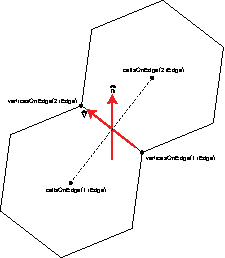
\includegraphics[height=3.5in]{shared_figures/angleEdge.pdf}
\caption{The angle of an edge refers to the angle between a vector pointing north at an edge location
and a vector pointing in the positive tangential velocity direction of the edge.}
\label{fig:angleEdge}
\end{center}
\end{figure}

The angle of each edge in an MPAS grid is provided in the variable {\it angleEdge}. The angle
given is the angle between a vector pointing north and a vector pointing in the
positive tangential direction of the edge. Referring to Fig. \ref{fig:angleEdge},
\[ {\rm angleEdge} = \arcsin\|{\bf \hat n} \times {\bf \hat v}\|, \]
where ${\bf \hat n}$ is the unit vector pointing north and ${\bf \hat v}$ is the unit vector
pointing from verticesOnEdge(1,iEdge) to verticesOnEdge(2,iEdge).

Given a wind vector $(u_\perp, u_\parallel)$ defined in term of components orthogonal to
and parallel to the edge, the earth-relative wind $(u,v)$ may be recovered as
\[
\begin{bmatrix}
u \\
v \\
\end{bmatrix}
=
\begin{bmatrix}
\cos\alpha && -\sin\alpha \\
\sin\alpha && \cos\alpha \\
\end{bmatrix}
\begin{bmatrix}
u_\perp \\
u_\parallel \\
\end{bmatrix},
\]
where $\alpha = {\rm angleEdge}$.





%--------------------------------------------------------------------------------------------
% Plotting model output
%--------------------------------------------------------------------------------------------

\chapter{Visualization}
\label{chap:mpas_visualization}

This chapter discusses visualization tools that may be used by all cores.  For instructions on additional visualization tools for this core, see Chapter \ref{chap:\core_visualization}.

\section{ParaView}

ParaView may be used to visualize MPAS initialization, output, and restart files.  It includes a reader that was specifically designed to read MPAS NetCDF files, including Cartesian and spherical domains.  At this time, only cell-centered quantities may be plotted with ParaView.  Variables located at edges and vertices must be interpolated to cell centers for visualization.

ParaView is freely available for download at \url{http://www.paraview.org}.  Binary installations are available for Windows, Mac, and Linux, as well as source code files and tutorials.  From the ParaView website:
\begin{quotation}
ParaView is an open-source, multi-platform data analysis and visualization application. ParaView users can quickly build visualizations to analyze their data using qualitative and quantitative techniques. The data exploration can be done interactively in 3D or programmatically using ParaView's batch processing capabilities.  ParaView was developed to analyze extremely large datasets using distributed memory computing resources. It can be run on supercomputers to analyze datasets of terascale as well as on laptops for smaller data.
\end{quotation}

To visualize an MPAS cell-centered variable in ParaView, open the file and choose {\tt MPAS NetCDF (Unstructured)} as the file format.  In the lower left Object Inspector panel, choose your variables of interest (Figure \ref{fig:ParaviewExample}).  For large data sets, loading fewer variables will result in less wait time.  Options are available for latitude-longitude projections, vertical level, etc.  Click the 'Apply' button to load the data set.  In the toolbars at the top, choose the variable to plot from the pull-down menu, and 'Surface' for the type of visualization.  The color bar button displays a color bar, and the color scale editor button allows the user to manually change the color bar type and extents.  The Filters menu provides computational tools for interactive data manipulation.  Movies, in avi format or as individual frames, may be conveniently created with the {\tt Save Animation} tool in the File menu.


\begin{figure}[htb]
\begin{center}
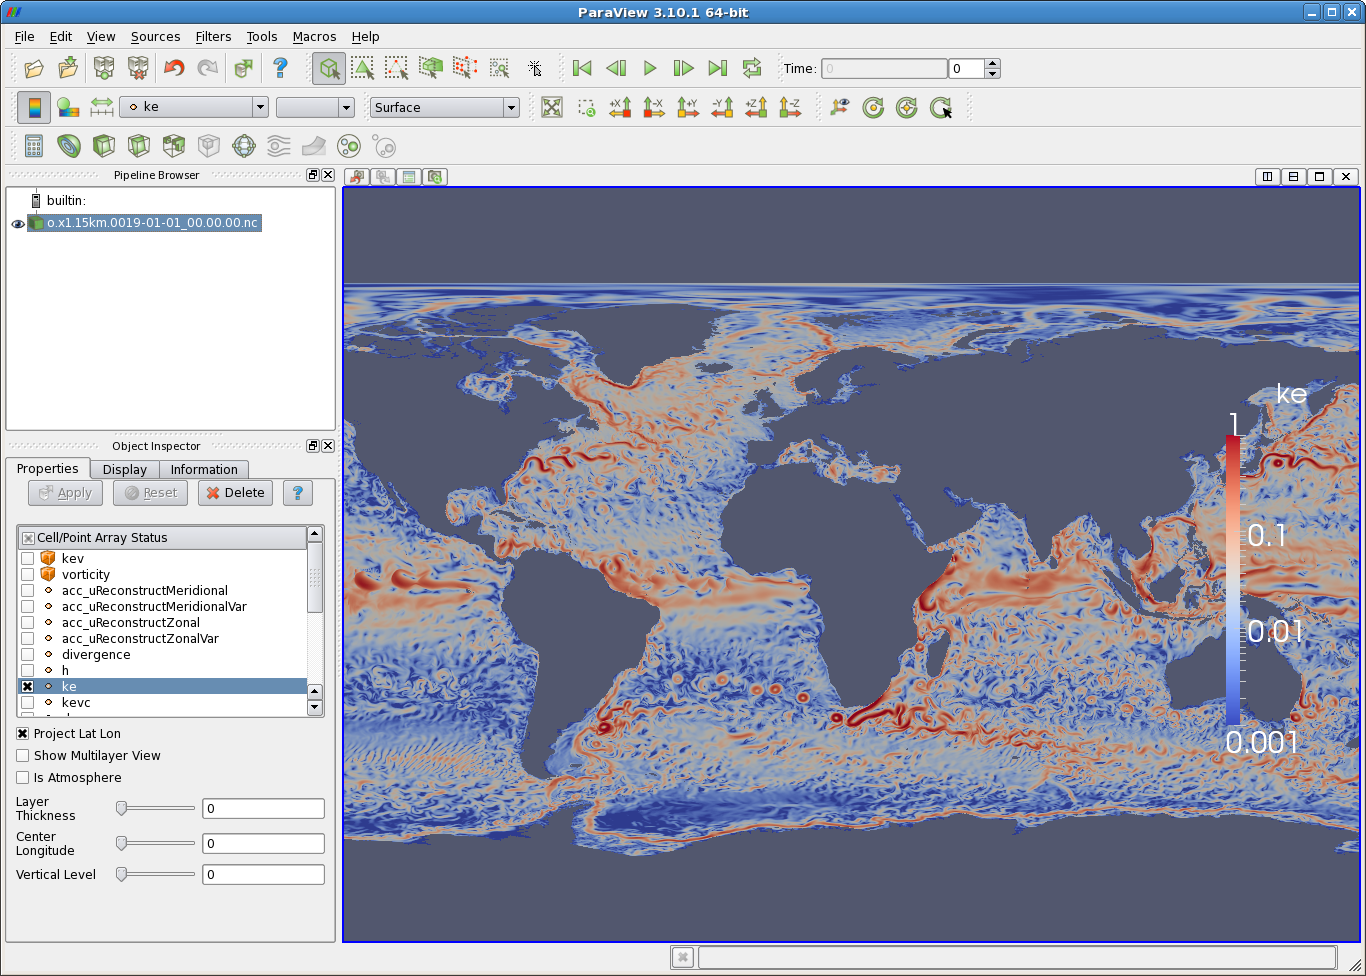
\includegraphics[width=6.5in]{shared/figures/ParaviewExample.png}
\caption{Example of ParaView to view an MPAS NetCDF file.}
\label{fig:ParaviewExample}
\end{center}
\end{figure}

%\appendix{Generating meshes}
\label{chap:mpas_grid_generation}

This chapter describes the steps used to create the  spherical centroidal Voronoi tessellation (SCVT) meshes and mesh-decomposition files used by MPAS models.
Since it can take considerable time (often several days or more) to generate a mesh as described in \S \ref{sec:global_scvt}, it is recommended to obtain 
and use existing SCVT meshes from \url{http://www.mmm.ucar.edu/people/duda/mpas/} whenever possible; these meshes can be quickly
modified to shift or rotate the refinement regions over the geographic areas of interest using the utility program described in \S \ref{sec:grid_rotate}.

\section{Density functions}

In all MPAS models, the horizontal meshes are SCVTs with a C-grid staggering of
velocities. As their name suggests, SCVTs are Voronoi tessellations defined on the surface of a sphere, and in which the generating 
point for each Voronoi region is also the mass centroid of that region with respect to some {\em density function}. An overview of
the application of SCVTs to multi-resolution climate modeling is given in Ringler et al. (2008)
\footnote{Ringler, T., L. Ju and M. Gunzburger, 2008, A multiresolution method for climate system modeling: application of spherical centroidal Voronoi tessellations, {\em Ocean Dynamics}, 58 (5-6), 475-498. doi:10.1007/s10236-008-0157-2.}.

For the purposes of generating SCVTs, the central concern lies with the density function, $\rho$, which is a user-defined
function relating the relative resolutions in different regions of the mesh. Specifically, for two generating points of the 
SCVT, ${\bf x}_i$ and ${\bf x}_j$,
\[
{h_i \over h_j} \approx \left({\rho({\bf x}_j) \over \rho({\bf x}_i)} \right)^{1 \over 4},
\]
where $h_i$ and $h_j$ are the diameters of the Voronoi cells associated with ${\bf x}_i$ and ${\bf x}_j$, respectively.

In the mesh generation program global\_scvt, described in the next section, the density function is defined programatically in the Fortran function
{\tt density\_for\_point()}, which returns the value of the density function, $\rho({\bf x})$, given a location on the sphere, ${\bf x}$.
   
\section{The global\_scvt program}
\label{sec:global_scvt}

\subsection{Compilation}
                                                                                             
As a first step toward building the global\_scvt code, the environment variable                     
{\tt NETCDF} must be set to the root of the netCDF installation. Unlike with the MPAS model, separate make targets are not
defined for each compiler set, and it will generally be necessary to edit the top-level Makefile to set the compiler and compiler flags                 
that will be used to build global\_scvt; however, there are commented-out sections in the Makefile for using either of the ifort, pgf90, or gfortran compilers that may be uncommented or used as a starting point for other compilers. Also, if the netCDF installation has a separate Fortran interface library, {\tt -lnetcdff} will need to be added before {\tt -lnetcdf} in the Makefile. The global\_scvt program is parallelized with OpenMP, so if compiler support is available, OpenMP compiler flags may be added
in the Makefile as well.                      

Before compiling the global\_scvt program, a density function should first be defined in the function {\tt density\_for\_point()} in {\tt src/module\_scvt.F}. The default density function is a uniform density function that returns a value of 1.0 for all locations
on the sphere, and commented code in {\tt density\_for\_point()} may be uncommented to achieve an area of circular refinement. {\em Note that, although $\rho({\bf x})$ could in principle take on any non-negative value, the code to scale eddy viscosities by the mesh resolution in the MPAS model assumes that $\rho({\bf x}) \in (0,1]$, so care should be taken when designing a new density function: a value of 1.0 should correspond to the highest-resolution regions(s) in the mesh.}                                      
                                                                                                
After editing the Makefile and defining the desired density function, running `make' should create the grid\_gen executable 
in the top-level directory. A second program, grid\_ref, may also be created, but this program is not needed by the current version 
of the global\_scvt program.

\subsection{Running}

As will be described in Section \ref{sec:grid_gen_efficiency}, a typical mesh is generated using multiple refinement steps. Within each of these steps, an SCVT with a fixed
number of generating points is converged before the SCVT is refined, giving a larger number of generating points to begin the next step. In this section, the process of converging an SCVT within a single step is described.

Two files are needed in order to run the grid\_gen program: an initial generating point file, {\tt locs.dat}, and a                        
namelist file, {\tt namelist.input}. The {\tt locs.dat} file contains a list of the Cartesian coordinates (assuming a unit-radius sphere
centered at the origin) of each of the beginning generating points, and the {\tt namelist.input} file specifies the number of generating points to be read from the {\tt locs.dat} file, the number of iterations to run, and the convergence criteria; a complete list of namelist variables is provided in the table below.

\vspace{12pt}
\begin{longtable}{|p{1.25in} |p{4.5in}|}
\hline
np & the number of points to read from the {\tt locs.dat} file \\ \hline
locs\_as\_xyz & whether the initial generating points in {\tt locs.dat} are given in Cartesian space ({\tt .true.}) or latitude-longitude space ({\tt .false.}) \\ \hline
n\_scvt\_iterations & the maximum number of Lloyd iterations to perform \\ \hline
eps & the convergence criterion, specifying the maximum permissible average movement of a generating point during an iteration \\ \hline
l2\_conv & whether to stop iterating if the convergence criterion is met \\ \hline
inf\_conv & currently the same meaning as l2\_conv \\ \hline
min\_dx & the targeted minimum grid distance in the mesh, on which an estimate for the number of generating points will be based; see Section \ref{sec:estimating_np} \\ \hline
\end{longtable}
\vspace{12pt}

\noindent A convergence criterion of $1\times10^{-10}$ should be sufficient, and in                     
practice, many thousands of iterations are needed to reach this tolerance.

If grid\_gen was compiled with OpenMP support, the environment variable {\tt OMP\_NUM\_THREADS} can be set to the 
number of threads that will be used by the program. Then, grid\_gen can be run with no command-line arguments:

\vspace{12pt}
{\tt > ./grid\_gen}
\vspace{12pt}
                                                                                         
                                                                                                
When grid\_gen finishes --- either because the convergence criterion has been met, or the
maximum number of iterations have been performed ---  several output files should be created: 

\begin{itemize}
\item {\tt scvt\_initial.ps} --- a plot of the mesh at the start of iterations,
\item {\tt scvt\_final.ps} --- a plot of the mesh after iterations,
\item {\tt grid.nc} --- the actual MPAS mesh file, which can be used with the initialization core to create an MPAS input file,
\item {\tt graph.info} --- information describing the cell connectivity graph of the mesh, to be used with a graph partitioner as described in Section \ref{sec:metis}, and
\item {\tt locs.dat.out} --- a list of the final generating points appended with a set of $3 np - 6$ refinement points. 
\end{itemize}

If the tolerance specified in the {\tt namelist.input} file was met, the SCVT mesh should be sufficiently converged, and the resulting {\tt grid.nc}
file can be used with the initialization program to create an initial condition file for MPAS; alternatively, the full set of $4 np - 6$ refinement points in 
the {\tt locs.dat.out} file can be used as input to the grid\_gen program to create another SCVT with approximately twice the resolution. If, however, the specified tolerance was not met, the {\tt locs.dat.out} file may be copied to {\tt locs.dat}, and further iteration may be performed on the SCVT.

To create a plot of the mesh with coastlines, which can be helpful when locating or sizing refinement regions, the {\tt mesh.ncl} script may be used to plot the mesh directly from                 
the {\tt grid.nc} file.                                                                          

\subsection{Estimating the required number of generating points}
\label{sec:estimating_np}

Setting the {\tt min\_dx} variable in the {\tt namelist.input} file to the targeted minimum grid distance in the mesh and running the grid\_gen program will cause the program to print out an estimate for the number of generating points that will be required to achieve that minimum grid distance with the density function provided in {\tt density\_for\_point()}.

\subsection{Efficiency concerns}
\label{sec:grid_gen_efficiency}

Although one could, given an estimate for the number of generating points needed to achieve the required absolute resolutions in the mesh,
create a {\tt locs.dat} file with that number of randomly chosen points on the unit sphere, and, using that {\tt locs.dat} file, converge a final SCVT, 
experience indicates that a stepwise approach can significantly reduce the required wallclock time.                   

   
\section{The grid\_rotate program} 
\label{sec:grid_rotate} 

The purpose of the grid\_rotate program is simply to rotate an MPAS mesh file, moving a refinement region from one geographic location to another, so that the mesh can be re-used for different applications. This utility was developed out of the need to save computational resources, since generating an SCVT --- particularly one with a large number of generating points or a high degree of refinement --- can take considerable time.

To build the grid\_rotate program, the Makefile should first be edited to set the Fortran compiler to be used; if the netCDF installation pointed to by the {\tt NETCDF} environment variable was build with a separate Fortran interface library, it will also be necessary to add {\tt -lnetcdff} just before {\tt -lnetcdf} in the Makefile. After editing the Makefile, running `make' should result in a grid\_rotate executable file.

Besides the MPAS grid file to be rotated, grid\_rotate requires a namelist file, {\tt namelist.input}, which specifies the rotation to be applied to the mesh. The namelist variables are summarized in the table below
   
\vspace{12pt}
\begin{longtable}{|p{3.25in} |p{2.5in}|}
\hline
config\_original\_latitude\_degrees & original latitude of any point on the sphere \\ \hline
config\_original\_longitude\_degrees & original longitude of any point on the sphere \\ \hline
config\_new\_latitude\_degrees &  latitude to which the original point should be shifted \\ \hline
config\_new\_longitude\_degrees &  longitude to which the original point should be shifted \\ \hline
config\_birdseye\_rotation\_counter\_clockwise\_degrees & rotation about a vector from the sphere center through the original point \\ \hline
\end{longtable}
\vspace{12pt}

\noindent Essentially, one chooses any point on the sphere, decides where that point should be shifted to,
and specifies any change to the orientation (i.e., rotation) of the mesh about that point. 

Having set the rotation parameters in the {\tt namelist.input} file, the grid\_rotate program should be run with two command-line options
specifying the original grid file name and the name of the rotated grid file to be produced, e.g.,

\vspace{12pt}
{\tt > grid\_rotate grid.nc grid\_SE\_Asia\_refinement.nc}
\vspace{12pt}

The original grid file will not be altered, and a new, rotated grid file will be created. The NCL script {\tt mesh.ncl} may be used to plot either of the original or rotated grid files after suitable setting the name of the grid file in the script.
   
   
\section{Graph partitioning with METIS} 
\label{sec:metis}

{\color{red} THIS SECTION WAS COPIED TO mpas_build_instructions.tex  FOR RELEASE 1.0. WHEN GRID GENERATION IS INCLUDED, DELETE THE METIS SECTION FROM mpas_build_instructions.tex}.

Before MPAS can be run in parallel, a mesh decomposition file with an appropriate number of 
partitions (equal to the number of MPI tasks that will be used) is required in the run directory.  A limited number of mesh decomposition files ({\tt graph.info.part.*}) are provided with each test case (see Test Cases Chapter).  In order to create new mesh decomposition files for your desired number of partitions, begin with the {\tt graph.info} file created by the grid\_gen program or available with your test case, and partition with METIS software (\url{http://glaros.dtc.umn.edu/gkhome/views/metis}). The serial graph partitioning program, METIS (rather than ParMETIS or hMETIS) should be sufficient for quickly partitioning any SCVT produced by the grid\_gen mesh generator.

After installing METIS, a {\tt graph.info} file may be partitioned into $N$ partitions by running

\vspace{12pt}
{\tt > gpmetis graph.info} $N$
\vspace{12pt}

\noindent The resulting file, {\tt graph.info.part.}$N$, can then be copied into the MPAS run directory
before running the model with $N$ MPI tasks.



\part{Non-hydrostatic Atomospheric Core}
%--------------------------------------------------------------------------------------------
% Running the MPAS non-hydrostatic atmosphere model
%--------------------------------------------------------------------------------------------

\chapter{Running the MPAS non-hydrostatic atmosphere model}

\setlength\LTleft{0.0in}

Given an SCVT mesh, this chapter describes the two main steps to running the non-hydrostatic model: creating initial conditions and running the model itself.  This chapter makes use of two MPAS cores, {\tt init\_atmosphere} and {\tt atmosphere}, which are, respectively, used for initializing and running the non-hydrostatic atmospheric model.  Sections 3.1 and 3.2 of this chapter describe the creation of idealized and real-data non-hydrostatic initial condition files using the {\tt init\_atmosphere} core.   Section 3.3 describes the basic procedure of running the model itself.

Each section of this chapter follows a familiar pattern of compiling and executing MPAS model components, albeit using different cores depending on its intended use.  The compilation will create either an initialization or a model executable, which are named, respectively, {\tt init\_atmosphere\_model} and {\tt atmosphere\_model}.  In general, if an MPAS executable was compiled for serial use, simply call the executable by name. If compiled to be run in parallel, the executable is called with {\tt mpiexec} or {\tt mpirun}, for example:

\vspace{12pt}
{\tt > mpiexec -n 8 atmosphere\_model}
\vspace{12pt}


\noindent where {\tt 8} is the number of MPI tasks to be used.  In any case where {\tt n} $>$ 1, there must exist a corresponding graph decomposition file, e.g., {\tt graph.info.part.8}. For more on graph decomposition, see \S 2.4.  

\section{Creating idealized ICs}

There are several idealized test cases supported within the {\tt init\_atmosphere} model initialization core:

1 --- Jablonowski and Williamson baroclinic wave, no initial perturbation
\footnote{Jablonowski, C. and D.L. Williamson, 2006, A baroclinic instability test case for atmospheric model dynamical cores, {\em QJRMS}, 132, 2943-2975. doi:10.1256/qj.06.12.}

2 --- Jablonowski and Williamson baroclinic wave, with initial perturbation

3 --- Jablonowski and Williamson baroclinic wave, with normal-mode perturbation

4 --- squall line

5 --- super-cell

6 --- mountain wave\\
\\
Creating idealized initial conditions is fairly straightforward, as no external data are required and the starting date/time is irrelevant to building the {\tt init.nc} file that will be used to run the model.

The following steps summarize the creation of {\tt init.nc}:

\begin{itemize}
\item Include a {\tt grid.nc} file, which contains the SCVT mesh, in the working directory (\S 2)
\item If running in parallel, include a {\tt graph.info.part.*} file in the working directory (\S 2.4)
\item Compile MPAS with the {\tt init\_atmosphere} core specified (\S 1.2)
\item Create an appropriate {\tt namelist.input} configuration file (described below)
\item Run {\tt init\_atmosphere\_model} to create {\tt init.nc}
\end{itemize}~\\

Included in the MPAS directory is a sample initialization namelist, {\tt namelist.input.init\_atmosphere}, which can be copied or linked to the {\tt namelist.input} file for use in this step.  A number of the namelist parameters found in {\tt namelist.input.init\_atmosphere} are irrelevant to creating idealized conditions and can be removed or ignored.  The following table outlines the namelist parameters that are required; comments are given on the right for certain key parameters, and formal explanations for all namelist parameters can be found in Appendix A.


\begin{longtable}{p{3in}|p{3.25in}}

\&nhyd\_model\\
   config\_init\_case       = 1                      & a number between 1 and 6 corresponding to the cases listed at the beginning of this section\\
   config\_theta\_adv\_order = 3                     & advection order for theta \\
/\\
\\
\&dimensions\\
   config\_nvertlevels     = 41                      & the number of vertical levels to be used in the model \\
/\\
\\
\&io\\
   config\_input\_name         = 'grid.nc'           & the name of the netCDF grid file from \S2 \\
   config\_output\_name        = 'init.nc'           & the name of the IC file to be created \\
/\\
\\
\&decomposition\\
   config\_block\_decomp\_file\_prefix = 'graph.info.part.' & if running in parallel, needs to match the grid decomposition file prefix \\
/\\

\end{longtable}



\section{Creating real-data ICs}

Creating real-data initial conditions is similar to that of the idealized case described in the previous section, but is more involved as it requires interpolation of static geographic data (e.g., topography, land cover, soil category, etc.), surface fields such as SST, and the atmospheric initial conditions associated with a particular date/time.  The static datasets are the same as those used by the WRF model, and the surface fields and atmospheric initial conditions can be obtained from GFS data using the WRF pre-processing system (WPS).

Creating real-data initial conditions requires a single compilation of the {\tt init\_atmosphere} core, but the actual generation of the IC files will take place using three separate runs of {\tt init\_atmosphere}, where each of these runs is described individually in the following sub-sections.  While it is possible to condense the three real-data initialization steps into fewer executions, running each step separately will both improve clarity and, as will become apparent, save a significant amount of time when generating subsequent initial conditions, that is, when making initial conditions using the same mesh but different starting times.

The first of the three steps, described in \S 3.2.1, is the interpolation of static fields onto the mesh to create a {\tt static.nc} file.  This step cannot be run in parallel and takes considerably longer than the steps that follow, however, the fields being static, this step need only be run once for a particular mesh, regardless of the number of initial condition files that are ultimately created from the {\tt static.nc} output file.  Described in \S 3.2.2 is an optional step that creates a file {\tt surface.nc} that contains surface data at regular intervals. This file is used in the case where the model run makes periodic external updates to surface fields (currently only sea-ice and SST).  Finally, \S 3.2.3 describes the processing of the atmospheric initial conditions beginning with the {\tt static.nc} file created in \S 3.2.1.  Naturally, each of the initialization runs described in the three following sections will make use of a {\tt namelist.input} file, and as was the case for idealized initial conditions, the file {\tt namelist.input.init\_atmosphere} in the MPAS directory can be used as a starting point.  Not every variable in this namelist is needed for any particular step, and therefore each section will elaborate only on the namelist variables that are immediately relevant.

\subsection{Static fields}

The generation of a file {\tt static.nc} requires a set of static geographic data.  A suitable dataset can be obtained from the WRF model's download page \\
 \url{http://www.mmm.ucar.edu/wrf/users/download/get\_source.html}.  These static data files should be downloaded to a directory, which will be specified the {\tt namelist.input} file (described below) prior to running this interpolation step.  The result of this run will be the creation of a netCDF file ({\tt static.nc}), which is used in the two steps, described in \S 3.2.2 and \S 3.2.3, following this to create surface update files and dynamic initial conditions.  Note that {\tt static.nc} can be generated once and then used repeatedly to generate surface update and initial condition files for different start times.

The following steps summarize the creation of {\tt static.nc}:

\begin{itemize}
\item Download geographic data from the WRF download page (described above) 
\item Compile MPAS with the {\tt init\_atmosphere} core specified (\S 1.2)
\item Include a {\tt grid.nc} file in the working directory (\S 2)
\item Create an appropriate {\tt namelist.input} configuration file (described below)
\item Run {\tt init\_atmosphere\_model} {\em either in serial or with only one MPI task specified} to create {\tt static.nc}
\end{itemize}~\\
Note that it is critical for this step that the initialization core is run serially; if the core was compiled in parallel, one only MPI task must be used ({\tt mpiexec -n 1 init\_atmosphere\_model}).  The steps described in \S 3.2.2 and \S 3.2.3 may be run in serial or parallel.

\begin{longtable}{p{3.0in} |p{3.25in}}

\&nhyd\_model\\
   config\_init\_case       = 7                      & must be 7, the real-data initialization case \\
/\\
\\
\&dimensions                                         & the following two variables must be present now, though their values do not become significant until \S 3.2.3 \\
   config\_nvertlevels     = 41                      &  \\
   config\_nsoillevels     = 4                       &  \\
/\\
\\
\&data\_sources\\
   config\_geog\_data\_path  = '/WPS\_GEOG/'         & absolute path to static files obtained from the WRF download page\\
/\\
\\
\&preproc\_stages                                    & only the static\_interp stage should be enabled \\
   config\_static\_interp   = .true.                 & \\
   config\_vertical\_grid   = .false.                & \\
   config\_met\_interp      = .false.                & \\
   config\_input\_sst       = .false.                & \\
/\\
\\
\&io\\
   config\_input\_name         = 'grid.nc'           & the name of the netCDF grid file from \S 2 \\
   config\_output\_name        = 'static.nc'         & file name for static netCDF output \\
/\\

\end{longtable}


\subsection{Surface field updates}

This step is optional --- it is required only if surface fields are to be periodically updated during the model run.  The surface data could originate from any number of sources, though the most straightforward way to obtain a dataset in the appropriate format is to process GRIB data (e.g., GFS GRIB data) with the {\em ungrib} program of the WRF model's pre-processing system (WPS).  Detailed instructions for building and running the WPS, and the process of generating intermediate data files from GFS data, can be found in Chapter 3 of the WRF User Guide: \url{http://www.mmm.ucar.edu/wrf/users/docs/user\_guide/users\_guide\_chap3.htm}.

The following steps summarize the creation of {\tt surface.nc}:

\begin{itemize}
\item Include surface data intermediate files in the working directory
\item Include a {\tt static.nc} file in the working directory (\S 3.2.1)
\item If running in parallel, include a {\tt graph.info.part.*} in the working directory (\S 2.4)
\item Create an appropriate {\tt namelist.input} configuration file (see below)
\item Run {\tt init\_atmosphere\_model} to create {\tt surface.nc}
\end{itemize}


\begin{longtable}{p{3.0in} |p{3.25in}}

\&nhyd\_model\\
   config\_init\_case       = 8                      & must be 8, the surface field initialization case \\
   config\_start\_time      = '2010-10-23\_00:00:00' & time to begin processing surface data \\
   config\_stop\_time       = '2010-10-24\_00:00:00' & time to end processing surface data \\
/\\
\\
\&data\_sources\\
   config\_sfc\_prefix      = 'SST'                  & the prefix of the intermediate data files containing SST and sea-ice \\
   config\_fg\_interval     = 21600                  & interval between intermediate files to use for SST and sea-ice \\
/\\
\\
\\
\&preproc\_stages                                    & only the config\_input\_sst step should be enabled \\
   config\_static\_interp   = .false.                & \\
   config\_vertical\_grid   = .false.                & \\
   config\_met\_interp      = .false.                & \\
   config\_input\_sst       = .true.                 & \\
/\\
\\
\&io\\
   config\_input\_name          = 'static.nc'        & name of the netCDF static data file \S 3.2.1 \\
   config\_sfc\_update\_name    = 'surface.nc'       & surface-update file name \\
/\\
\\
\&decomposition\\
   config\_block\_decomp\_file\_prefix = 'graph.info.part.' & if running in parallel, needs to match the grid decomposition file prefix \\
/\\

\end{longtable}



\subsection{Vertical grid generation and initial field interpolation}

The final step for creating a real-data initial conditions file ({\tt init.nc}) is to generate a vertical grid, the parameters of which will be specified in the {\tt namelist.input} file, and to obtain an initial conditions dataset and interpolate it onto the model grid. As stated previously, while initial conditions could ultimately be obtained from many different data sources, here we assume the use of intermediate data files obtained from GFS data using the WPS ungrib program.  Detailed instructions for building and running the WPS, and how to generate intermediate data files from GFS data, can be found in Chapter 3 of the WRF user guide: \\
\url{http://www.mmm.ucar.edu/wrf/users/docs/user\_guide/users\_guide\_chap3.htm}.

The following steps summarize the creation of {\tt init.nc}:

\begin{itemize}
\item Include a WPS intermediate data file in the working directory
\item Include the {\tt static.nc} file in the working directory (\S 3.2.1)
\item If running in parallel, include a {\tt graph.info.part.*} file in the working directory (\S 2.4)
\item Create an appropriate {\tt namelist.input} configuration file (described below)
\item Run {\tt init\_atmosphere\_model} to create {\tt init.nc}
\end{itemize}


\begin{longtable}{p{3.0in} |p{3.25in}}

\&nhyd\_model\\
   config\_init\_case       = 7                      & must be 7 \\
   config\_theta\_adv\_order = 3                     & advection order for theta \\
   config\_start\_time      = '2010-10-23\_00:00:00' & time to process first-guess data \\
/\\
\\
\&dimensions\\
   config\_nvertlevels     = 41                      & number of vertical levels to be used in MPAS \\
   config\_nsoillevels     = 4                       & number of soil layers to be used in MPAS \\
   config\_nfglevels       = 38                      & number of vertical levels in intermediate file \\
   config\_nfgsoillevels   = 4                       & number of soil layers in intermediate file \\
/\\
\\
\&data\_sources\\
   config\_met\_prefix      = 'FILE'                 & the prefix of the intermediate file to be used for initial conditions \\
/\\
\\
\&vertical\_grid\\
   config\_ztop            = 30000.0                 & model top height (m) \\
   config\_nsmterrain      = 2                       & number of smoothing passes for terrain \\
   config\_smooth\_surfaces = .false.                 & whether to smooth zeta surfaces \\
/\\
\\
\&preproc\_stages                                    & \\
   config\_static\_interp   = .false.                & \\
   config\_vertical\_grid   = .true.                 & only these three stages should be enabled \\
   config\_met\_interp      = .true.                 & \\
   config\_input\_sst       = .false.                & \\
/\\
\\
\&io\\
   config\_input\_name         = 'static.nc'         & the netCDF static file \S 3.2.1 \\
   config\_output\_name        = 'init.nc'           & name of the IC file to be created \\
/\\
\\
\&decomposition\\
   config\_block\_decomp\_file\_prefix = 'graph.info.part.' & if running in parallel, needs to match the grid decomposition file prefix \\
/\\
\end{longtable}


\section{Running the model}

With the files {\tt init.nc} and, optionally, {\tt surface.nc}, generated as in the previous sections, we have completed the prerequisites to run the model.  The only step remaining before running the model itself is the configuration of {\tt namelist.input}.  As a starting point, the MPAS directory contains {\tt namelist.input.atmosphere}, along with three other namelists corresponding to the various idealized cases, that can be copied or linked to {\tt namelist.input}.  This section will discuss both running the model from a cold start and restarting the model from some point in a previous run.

The following steps summarize running the model:

\begin{itemize}
\item Include an initial condition netCDF file (e.g., {\tt init.nc}) in the working directory(\S 3.1, \S 3.2)
\item If using surface updates, include a surface netCDF file (e.g., {\tt surface.nc}) in the working directory (\S 3.2.2)
\item If running in parallel, include a graph decomposition file in the working directory (\S 2.4)
\item If the MPAS directory has not been cleaned since running initialization, run {\tt make clean} with the {\tt init\_atmosphere} core specified
\item Compile MPAS with the {\tt atmosphere} core specified (\S 1.2)
\item Create an appropriate {\tt namelist.input} configuration file (described below)
\item Run the compiled executable
\end{itemize}

Below is a list of variables in {\tt namelist.input} that pertain to input, output, and model restarts.  A number of namelist variables are not listed here (specifications for dynamical core configuration, physics parameters, etc.) and Appendix A should be consulted for the purpose and acceptable values of these parameters.

\begin{longtable}{p{3.0in} |p{3.25in}}

\&nhyd\_model                                        & \\
   config\_dt = 450.0                                & the model timestep; an appropriate value must be chosen relative to the grid cell spacing \\
   config\_start\_time = '2010-10-23\_00:00:00'      & the model start time corresponding to {\tt init.nc}\\
   config\_run\_duration = '5\_00:00:00'             & the duration of the model run; for format rules, see Appendix A \\
   config\_sfc\_update\_interval = 'none'            & the frequency of surface updates; for format rules, see Appendix A \\
/                                                    & \\
   config\_stop\_time  = '0000-01-16\_00:00:00'      & this can be used in place of {\tt config\_run\_duration} \\
                                                     & \\
\&io                                                 & \\
   config\_input\_name = 'init.nc'                   & the IC file from \S 3.1 or 3.2 \\
   config\_output\_name = 'output.nc'                & the name of the output netCDF file (if necessary, date/time will be inserted automatically) \\
   config\_restart\_name = 'restart.nc'              & the name given to restart files will that will be created (date/time will be inserted automatically) \\
   config\_output\_interval = '1\_00:00:00'          & the interval to write data to the output file\\
   config\_frames\_per\_outfile = 1                  & a non-negative integer; 0 specifies a single output file \\
   config\_sfc\_update\_name = 'surface.nc'          & only needed if using surface updates (file from \S 3.2.2) \\
/ 
\\
\&decomposition                                            & \\
   config\_block\_decomp\_file\_prefix = 'graph.info.part.' & if running in parallel, must match the prefix of the graph decomposition file \\
/                                                    & \\
\\
\&restart                                            & \\
   config\_restart\_interval = '1\_00:00:00'         & the interval to create restart files; for format rules, see Appendix A \\
   config\_do\_restart = .false.                     & if true, will select the appropriate {\tt restart.nc} file generated from a previous run \\
/ 
\end{longtable}

When running the model from a cold start, {\tt config\_start\_time} should match the time that was used when creating {\tt init.nc}, and the file names specified in the {\tt \&io} section should be present in the working directory.  The model output can be written to a single file, e.g., {\tt output.nc}, or written to multiple files differentiated by the date of the file's first output frame.  This behaviour is determined by the variable {\tt config\_frames\_per\_outfile}: if set to 0, all output will be written to the single file {\tt output.nc}, and any number greater than 0 determines the maximum number of output frames written per output file.  For example, given the namelist values displayed above, an output file would be written for each day of the model run and each file would contain a single output frame.  Dates are inserted automatically into the output file names, so the output would be {\tt output.2010-10-23\_00:00:00.nc, output.2010-10-24\_00:00:00.nc}, etc.  In this example, if {\tt config\_frames\_per\_outfile} were changed to 3, a new output file would be created every third day and each would contain three frames per file.

During the course of a model run, restart files are created at an interval specified by the namelist variable {\tt config\_restart\_interval}.  A unique restart file is created for each restart time, and as was the case when multiple output files are created, they are differentiated by the automatic insertion of the restart date in the filename.  For example, the namelist values listed above would create the files {\tt restart.2010-10-24\_00:00:00.nc, restart.2010-10-25\_00:00:00.nc}, etc. Unlike with history output files, no restart file is created at the model initial time.

Running the model from a restart file is similar to running the model from {\tt init.nc}.  The required changes are that {\tt config\_do\_restart} must be set to {\tt .true.} and {\tt config\_start\_time} must correspond to a restart file existing in the working directory.


%--------------------------------------------------------------------------------------------
% Description of model fields
%--------------------------------------------------------------------------------------------

\chapter{Description of model fields}

In this chapter, the fields required in an MPAS input file are described. The dimensionality of each field is given in the name
of each field, with the dimensions in C storage order (i.e., the fastest-varying dimension is outer-most).

\section{Field dimensions}

{\small
\begin{longtable}{|p{1.75in} |p{4.5in}|}
 \hline
        nSoilLevels      &   Number of soil layers \\ \hline
        nMonths         &   Constant value 12 \\ \hline
        StrLen          &   Length of strings \\ \hline
\end{longtable}
}

\section{Vertical grid fields}

{\small        
\begin{longtable}{|p{2.5in} |p{3.75in}|}
 \hline
        double hx(nCells, nVertLevelsP1)     & h\_s field used in smoothed terrain-following coordinate \\ \hline
        double zgrid(nCells, nVertLevelsP1)  & height (m) at vertical cell interfaces (i.e. at $w$ points) \\ \hline
        double rdzw(nVertLevels)                & 1/($\Delta \zeta$ between w-levels) \\ \hline
        double dzu(nVertLevels)                 & $\Delta \zeta$ between u-levels (layer centers) \\ \hline
        double rdzu(nVertLevels)                & 1/dzu \\ \hline
        double fzm(nVertLevels)                 & dzw$_{k-1}$ / dzu$_k$, level $k-1$ interp weight from \hfil \break $u$ to $w$ points \\ \hline
        double fzp(nVertLevels)                 & dzw$_k$ / dzu$_k$, level $k$ interp weight from $u$ to $w$ points \\ \hline
        double zx(nEdges, nVertLevelsP1)        & $\partial z / \partial x$ \\ \hline
        double zz(nCells, nVertLevelsP1)        & $\partial \zeta / \partial z$ \\ \hline
%        double \hfil\break zf(nEdges, TWO, nVertLevelsP1)   & coefficients for contribution from $U$ to $\Omega$ diagnosis  \\ \hline
%        double \hfil\break zf3(nEdges, TWO, nVertLevelsP1)  &  coefficients for 3rd-order contribution from $U$ to $\Omega$ \hfil\break diagnosis \\ \hline
        double \hfil\break zb(nEdges, TWO, nVertLevelsP1)   & coefficients for contribution from $U$ to $w$ diagnosis \\ \hline
        double \hfil\break zb3(nEdges, TWO, nVertLevelsP1)  & coefficients for 3rd-order contribution from $U$ to $\Omega$ \hfil\break diagnosis \\ \hline
\end{longtable}
}
   
\newpage        
\section{Initial fields}  

{\small     
\begin{longtable}{|p{2.5in} |p{3.75in}|}
 \hline
        char xtime(Time, StrLen)     & Time stamp for each time record of fields in the file \\ \hline
        double \hfil\break theta(Time, nCells, nVertLevels)      &        Potential temperature (K) \\ \hline
        double rho(Time, nCells, nVertLevels)        &        Dry density (kg m$^{-3}$) \\ \hline
        double u(Time, nEdges, nVertLevels)         & Normal wind velocity at edges (m s$^{-1}$) \\ \hline
        double \hfil\break w(Time, nCells, nVertLevelsP1)       & Vertical velocity at vertical cell faces (m s$^{-1}$) \\ \hline
        double qv(Time, nCells, nVertLevels)   &              Water vapor mixing ratio (kg kg$^{-1}$) \\ \hline
        double qc(Time, nCells, nVertLevels)   &              Cloud water mixing ratio (kg kg$^{-1}$) \\ \hline
        double qr(Time, nCells, nVertLevels)   &              Rain water mixing ratio (kg kg$^{-1}$) \\ \hline
        double ter(nCells)           &  Terrain height (m) \\ \hline
        int landmask(nCells)         &  Land-water mask (1=land, 0=water) \\ \hline
        int ivgtyp(nCells)           &  Vegetation type category \\ \hline
        int isltyp(nCells)           &  Soil type category \\ \hline
        double snoalb(nCells)        &  Annual maximum snow albedo \\ \hline
        double soiltemp(nCells)      &  Climatological average soil temperature \\ \hline
        double greenfrac(nCells, nMonths)    & Climatological monthly mean greeness fraction \\ \hline
        double shdmin(nCells)                & Annual minimum greeness fraction \\ \hline
        double shdmax(nCells)                & Annual maximum greeness fraction \\ \hline
        double albedo12m(nCells, nMonths)    & Climatological monthly mean background albedo \\ \hline
        double dss(nCells, nVertLevels)         & w-damping coefficient \\ \hline
        double dzs(Time, nCells, nSoilLevels)       & Thickness of soil layers (m) \\ \hline
        double zs(Time, nCells, nSoilLevels)        & Depth of center of soil layers (m) \\ \hline
        double \hfil\break sh2o(Time, nCells, nSoilLevels)      & Soil liquid water (m$^{3}$ m$^{-3}$) \\ \hline
        double \hfil\break smois(Time, nCells, nSoilLevels)     & Soil moisture (m$^{3}$ m$^{-3}$) \\ \hline
        double tslb(Time, nCells, nSoilLevels)      & Soil layer temperature (K) \\ \hline
        double tmn(Time, nCells)                    & Deep soil temperature (K) \\ \hline
        double skintemp(Time, nCells)               & Surface skin temperature (K) \\ \hline
        double sst(Time, nCells)                    & Sea-surface temperature (K) \\ \hline
        double snow(Time, nCells)                   & Snow water equivalent (kg m-2) \\ \hline
        double snowc(Time, nCells)                  & Flag indicating snow coverage (1 for snow; 0 otherwise) \\ \hline
        double snowh(Time, nCells)                  & Physical snow depth (m) \\ \hline
        double xice(Time, nCells)                   & Sea-ice fraction \\ \hline
        double seaice(Time, nCells)                 & Sea-ice mask (1 when xice $>$ 0, 0 otherwise) \\ \hline
        double vegfra(Time, nCells)                 & Vegetation fraction \\ \hline
        double sfc\_albbck(Time, nCells)            &  Surface background albedo \\ \hline
        double xland(Time, nCells)                  & Land-ocean mask (1=land, 2=ocean) \\ \hline
        double qv\_init(nVertLevels)           &               qv reference profile \\ \hline
        double t\_init(nCells, nVertLevels)    &               theta reference profile for each cell \\ \hline
        double u\_init(nVertLevels)            &               u reference profile \\ \hline
        double coeffs\_reconstruct \hfil\break (nCells, maxEdges, R3) &   Coefficients for reconstructing wind vectors at cell centers. \\ \hline
        double defc\_b(nCells, maxEdges)                 & coefficients for computing the diagonal components \hfil\break of the horizontal deformation \\ \hline
        double defc\_a(nCells, maxEdges)                 &  coefficients for computing the off-diagonal components \hfil\break of the horizontal deformation\\ \hline
        int advCells(nCells, TWENTYONE)                  &indices of cells used to compute cell-centered 2nd derivatives for transport scheme \\ \hline
        double \hfil\break deriv\_two(nEdges, TWO, FIFTEEN)          & weights for cell centered 2nd derivatives, normal to edge, for the transport scheme \\ \hline
        double surface\_pressure(Time, nCells)           & Surface pressure (Pa) \\ \hline
        double \hfil\break theta\_base(Time, nCells, nVertLevels)    & Reference-state potential temperature (K) \\ \hline
        double \hfil\break rho\_base(Time, nCells, nVertLevels)      & Reference-state dry density (kg m$^{-3}$) \\ \hline
        double pressure\_base \hfil\break (Time, nCells, nVertLevels) & Reference-state dry pressure (Pa) \\ \hline
        double exner\_base \hfil\break (Time, nCells, nVertLevels)    & Reference-state Exner function (-) \\ \hline
        double fEdge(nEdges)         &  Coriolis parameter at edge locations \\ \hline
        double fVertex(nVertices)    &  Coriolis parameter at vertex locations \\ \hline
        double cf1                   &  surface interp weight for level $k=1$ values \\ \hline
        double cf2                   &  surface interp weight for level $k=2$ values \\ \hline
        double cf3                   &  surface interp weight for level $k=3$ values \\ \hline
\end{longtable}
}
        
\section{History fields}

{\small        
\begin{longtable}{|p{2.5in} |p{3.75in}|}
 \hline
        double v(Time, nEdges, nVertLevels)          &        Tangential wind velocity at edges (m s$^{-1}$)  \\ \hline 
        double uReconstructMeridional\hfil\break (Time, nCells, nVertLevels)  & Reconstructed meridional velocity at cell centers (m s$^{-1}$)  \\ \hline
        double uReconstructZonal\hfil\break (Time, nCells, nVertLevels)  &      Reconstructed zonal velocity at cell centers \hfil\break (m s$^{-1}$) \\ \hline
        double uReconstructZ\hfil\break (Time, nCells, nVertLevels)      &      Reconstructed z-component of velocity at cell centers \hfil\break (m s$^{-1}$) \\ \hline
        double uReconstructY\hfil\break (Time, nCells, nVertLevels)      &      Reconstructed y-component of velocity at cell centers \hfil\break (m s$^{-1}$) \\ \hline
        double uReconstructX\hfil\break (Time, nCells, nVertLevels)      &      Reconstructed x-component of velocity at cell centers \hfil\break (m s$^{-1}$)  \\ \hline
        double \hfil\break rho\_zz(Time, nCells, nVertLevels)   &  Dry density divided by d(zeta)/dz \\ \hline
        double \hfil\break theta\_m(Time, nCells, nVertLevels)  &  Modified moist potential temperature (K) \\ \hline
        double qsat \hfill\break(Time,nCells,nVertLevels) & Saturation mixing ratio  (kg kg$^{-1}$ ) \\ \hline
        double relhum \hfill\break(Time,nCells,nVertLevels) & Relative humidity (-) \\ \hline
\end{longtable}
}


\subsection{Cloud microphysics schemes}

{\small
\begin{longtable}{|p{2.0in} |p{3.5in} |p{0.5in} |}
\hline
        double rainncv (Time,nCells) & Time-step total precipitation due to microphysics & mm \\ \hline
        double snowncv (Time,nCells) & Time-step precipitation of snow due to microphysics & mm \\ \hline
        double graupelncv (Time,nCells) & Time-step precipitation of graupel due to microphysics & mm \\ \hline
        double rainnc (Time,nCells) & Accumulated total precipitation due to microphysics & mm \\ \hline
        double snownc (Time,nCells) & Accumulated precipitation of snow due to microphysics & mm \\ \hline
        double graupelnc (Time,nCells) & Accumulated precipitation of graupel due to microphysics & mm \\ \hline
        double sr (Time,nCells) & Ratio frozen to total precipitation due to microphysics & - \\ \hline
\end{longtable}
}

\subsection{Convection schemes}

{\small
\begin{longtable}{|p{2.0in} |p{3.0in} |p{1.0in} |}
\hline
        double cuprec (Time,nCells) & Time-step total precipitation rate due to convection & (mm day$^{-1}$) \\ \hline
        double raincv (Time,nCells)  & Time-step total precipitation due to convection & (mm) \\ \hline
        double rain (Time,nCells)      & Accumulated total precipitation due to convection & (mm) \\ \hline
        double rqccuten \hfil\break (Time,nCells,nVertLevels) & Tendency of cloud water due to convection &  (kg kg$^{-1}$ s$^{-1}$) \\ \hline
        double rqicuten \hfil\break (Time,nCells,nVertLevels) & Tendency of cloud ice due to convection & (kg kg$^{-1}$ s$^{-1}$) \\ \hline
        double rqvcuten \hfil\break (Time,nCells,nVertLevels) & Tendency of water vapor due to convection & (kg kg s$^{-1}$) \\ \hline
        double rthcuten \hfil\break (Time,nCells,nVertLevels) & Tendency of potential temperature due to convection & (K s$^{-1}$) \\ \hline
        double rqvdynten \hfil\break (Time,nCells,nVertLevels) & Tendency of water vapor due to total dynamical advection & (kg kg s$^{-1}$)\\ \hline
        \multicolumn{3}{|l|}{{\rule[-3mm]{0mm}{8mm}\bf KAIN-FRITSCH SCHEME SPECIFICS:} \hfill}\\ \hline
         double nca (Time,nCells) & Lifetime of convective clouds & (s) \\ \hline
        double cubot (Time,nCells) & Index level of cloud base for convective clouds & (-) \\ \hline
        double cutop (Time,nCells) & Index level of cloud top for convective clouds & (-) \\ \hline
        double wavg0 \hfil\break (Time,nCells,nVertLevels) & Temporal running-average vertical velocity & (m s$^{-1}$) \\ \hline
        double rqrcuten \hfil\break (Time,nCells,nVertLevels) & Tendency of rain due to convection &  (kg kg$^{-1}$ s$^{-1}$) \\ \hline
        double rqscuten \hfil\break (Time,nCells,nVertLevels) & Tendency of snow due to convection & (kg kg$^{-1}$ s$^{-1}$) \\ \hline
        \multicolumn{3}{|l|}{{\rule[-3mm]{0mm}{8mm}\bf TIEDTKE SCHEME SPECIFICS:} \hfill}\\ \hline
        double rucuten \hfil\break (Time,nCells,nVertLevels) & Tendency of zonal wind due to convection & (m s$^{-1}$ s$^{-1}$) \\ \hline
        double rvcuten \hfil\break (Time,nCells,nVertLevels) & Tendency of meridional wind due to convection & (m s$^{-1}$ s$^{-1}$) \\ \hline
\end{longtable}
}

\subsection{Planetary boundary (PBL) schemes}

{\small
\begin{longtable}{|p{2.0in} |p{3.0in} |p{1.0in}|}
\hline
integer kpbl (Time,nCells)  & Index level of PBL top & (-) \\ \hline
double hpbl (Time,nCells)  & Height of PBL top & (m) \\ \hline
double rublten \hfil\break (Time,nCells,nVertLevels)  & Tendency of zonal wind due to PBL processes  & (m s$^{-1}$ s$^{-1}$) \\ \hline
double rvblten \hfil\break (Time,nCells,nVertLevels)  &  Tendency of meridional wind due to PBL processes & (m s$^{-1}$ s$^{-1}$) \\ \hline
double rthblten  \hfil\break (Time,nCells,nVertLevels)  &  Tendency of potential temperature due to PBL processes& (K s$^{-1}$) \\ \hline
double rqvblten \hfil\break (Time,nCells,nVertLevels)  &  Tendency of water vapor due to PBL processes & (kg kg$^{-1}$ s$^{-1}$) \\ \hline
double rqcblten \hfil\break (Time,nCells,nVertLevels)  &  Tendency of cloud water due to PBL processes & (kg kg$^{-1}$ s$^{-1}$) \\ \hline
double rqiblten \hfil\break (Time,nCells,nVertLevels)  &  Tendency of cloud ice due to PBL processes & (kg kg$^{-1}$ s$^{-1}$) \\ \hline
\end{longtable}
}

\subsection{Horizontal cloud fraction}

{\small
\begin{longtable}{|p{2.0in}|p{3.0in}|p{1.0in}|}
\hline
double cldfrac \hfil\break (Time,nCells,nVertLevels) & Cloud fraction & (-)\\ \hline
\end{longtable}
}

\subsection{Radiation schemes}

{\small
\begin{longtable}{|p{2.0in} |p{3.0in} |p{1.0in} |}
\hline
\multicolumn{3}{|l|}{{\rule[-3mm]{0mm}{8mm}\bf SHORT-WAVE RADIATION SCHEMES:} \hfill}\\ \hline
double coszr  (Time,nCells) & Cosine of solar zenith angle & (-) \\ \hline
double gsw (Time,nCells) & SFC all-sky net shortwave radiation & (W m$^{-2}$) \\ \hline
double swdnb (Time,nCells) & SFC all-sky downward shortwave radiation & (W m$^{-2}$) \\ \hline
double swdnbc (Time,nCells) & SFC clear-sky downward shortwave radiation & (W m$^{-2}$) \\ \hline
double swupb (Time,nCells) & SFC all-sky upward shortwave radiation & (W m$^{-2}$) \\ \hline
double swupbc (Time,nCells) & SFC clear-sky upward shortwave radiation & (W m$^{-2}$) \\ \hline
double swdnt (Time,nCells) & TOA all-sky downward shortwave radiation & (W m$^{-2}$) \\ \hline
double swdntc (Time,nCells) & TOA clear-sky downward shortwave radiation & (W m$^{-2}$) \\ \hline
double swupt (Time,nCells) & TOA all-sky upward shortwave radiation & (W m$^{-2}$) \\ \hline
double swuptc (Time,nCells) & TOA clear-sky upward shortwave radiation & (W m$^{-2}$) \\ \hline
double swcf (Time,nCells) & TOA all-sky shortwave radiative cloud forcing & (W m$^{-2}$) \\ \hline
double rthratensw \hfil\break (Time,nCells,nVertLevels) & Tendency of potential temperature due to all-sky SW radiation & (K s$^{-1}$) \\ \hline

\multicolumn{3}{|l|}{{\rule[-3mm]{0mm}{8mm}\bf LONG-WAVE RADIATION SCHEMES:} \hfill}\\ \hline
double glw (Time,nCells)  & SFC all-sky net longwave radiation & (W m$^{-2}$) \\ \hline
double lwdnb (Time,nCells)  & SFC all-sky downward longwave radiation & (W m$^{-2}$) \\ \hline
double lwdnbc (Time,nCells)  & SFC clear-sky downward longwave radiation & (W m$^{-2}$) \\ \hline
double lwupb (Time,nCells)  & SFC all-sky upward longwave radiation & (W m$^{-2}$) \\ \hline
double lwupbc (Time,nCells)  & SFC clear-sky upward longwave radiation & (W m$^{-2}$) \\ \hline
double lwdnt (Time,nCells)  & TOA all-sky downward longwave radiation & (W m$^{-2}$) \\ \hline
double lwdntc (Time,nCells) & TOA clear-sky downward longwave radiation & (W m$^{-2}$) \\ \hline
double lwupt (Time,nCells)  & TOA all-sky upward longwave radiation & (W m$^{-2}$) \\ \hline
double lwuptc (Time,nCells)  & TOA clear-sky upward longwave radiation & (W m$^{-2}$) \\ \hline
double lwcf (Time,nCells)  & TOA all-sky longwave radiative cloud forcing & (W m$^{-2}$) \\ \hline
double olrtoa (Time,nCells) & TOA outgoing longwave radiation & (W m$^{-2}$) \\ \hline 
double rthratenlw \hfil\break (Time,nCells,nVertLevels)  & Tendency of potential temperature due to all-sky LW radiation & (K s$^{-1}$) \\ \hline

\multicolumn{3}{|l|}{{\rule[-3mm]{0mm}{8mm}\bf CAM RADIATION SPECIFICS:} \hfill}\\ \hline
double absnxt \hfill\break(Time,nCells,cam\_dim1,nVertLevels)  & Total nearest layer absorptivity & (-) \\ \hline
double abstot  \hfill\break(Time,nCells,nVertLevelsP1,nVertLevelsP1) & Total absorptivity & (-) \\ \hline
double emstot  \hfil\break (Time,nCells,nVertLevelsP1) & Total emissivity & (-) \\ \hline
double pin (nOznLevels) & Prescribed pressure levels for ozone mixing ratio & (hPa) \\ \hline
double ozmixm \hfil\break (nMonths nOznLevels nCells) & Climatological monthly ozone mixing ratio & (kg kg$^{-1}$) \\ \hline
double m\_hybi & Matched hybi (need to rechecked) & (-) \\ \hline
double m\_ps  & Surface pressure from match on MPAS grid & (Pa) \\ \hline
double sul \hfill\break (Time,nCells,nAerLevels)  & Sulfate soluble (SUL) aerosol concentration & (kg m$^{-3}$) \\ \hline
double sslt \hfill\break (Time,nCells,nAerLevels)  & Sea-salt (SSLT) aerosol concentration & (kg m$^{-3}$) \\ \hline
double dust1 \hfil\break (Time,nCells,nAerLevels) & Dust type 1 (DUST1) aerosol concentration & (kg m$^{-3}$) \\ \hline
double dust2  \hfil\break (Time,nCells,nAerLevels) & Dust type 2 (DUST2) aerosol concentration & (kg m$^{-3}$) \\ \hline
double dust3 \hfil\break (Time,nCells,nAerLevels) & Dust type 3 (DUST3) aerosol concentration & (kg m$^{-3}$) \\ \hline
double dust4 \hfil\break (Time,nCells,nAerLevels) & Dust type 4 (DUST4) aerosol concentration & (kg m$^{-3}$) \\ \hline
double ocpho \hfil\break (Time,nCells,nAerLevels) & Hydrophobic organic carbon (OCPHO) aerosol concentration & (kg m$^{-3}$) \\ \hline
double bcpho \hfil\break (Time,nCells,nAerLevels) & Hydrophobic black carbon (BCPHO) aerosol concentration & (kg m$^{-3}$) \\ \hline
double ocphi \hfil\break (Time,nCells,nAerLevels) & Hydrophilic organic carbon (OCPHI) aerosol concentration & (kg m$^{-3}$) \\ \hline
double bcphi \hfil\break (Time,nCells,nAerLevels) & Hydrophilci black carbon (BCPHI) aerosol concentration & (kg m$^{-3}$) \\ \hline
double bg \hfill\break (Time,nCells,nAerLevels) & Background (BG) aerosol concentration & (kg m$^{-3}$) \\ \hline
double volc \hfill\break (Time,nCells,nAerLevels) & Volcanic (VOLC) aerosol concentration & (kg m$^{-3}$) \\ \hline
\end{longtable}
}

\subsection{Surface layer scheme}

{\small
\begin{longtable}{|p{2.0in} |p{3.0in} |p{1.0in} |}
\hline
double br (Time,nCells) & Bulk Richardson number & (-) \\ \hline
double cd (Time,nCells) & 10-meters drag coefficient & (-) \\ \hline
double cda (Time,nCells) & Drag coefficient at lowest model level & (-) \\ \hline
double chs (Time,nCells) & \em{To be defined as local. Will need to be removed from Registry} & \\ \hline
double chs2 (Time,nCells) & \em{To be defined as local. Will need to be removed from Registry} & \\ \hline
double cqs2 (Time,nCells) & \em{To be defined as local. Will need to be removed from Registry} & \\ \hline
double ck (Time,nCells) & 10-meters enthalpy exchange coefficient & (-) \\ \hline
double cka (Time,nCells) &  Enthalpy exchange coefficient at lowest model level & (-) \\ \hline
double cpm (Time,nCells) & \em{To be defined as local. Will need to be removed from Registry} & (-) \\ \hline
double flhc (Time,nCells) & Exchange coefficient for heat & (-) \\ \hline
double flqc (Time,nCells) & Exchange coefficient for moisture & (-) \\ \hline
double gz1oz0 (Time,nCells) & Log of z1 over z0 & (-) \\ \hline
double hfx (Time,nCells) & Surface upward heat flux & (W m$^{-2}$) \\ \hline
double lh (Time,nCells) & Surface latent heat flux & (W m$^{-2}$) \\ \hline
double mavail (Time,nCells) & Surface moisture availability & (-) \\ \hline
double mol (Time,nCells) &  T$^{*}$ in similarity theory & (K) \\ \hline
double psim (Time,nCells) & Similarity function for heat & (-) \\ \hline
double psih (Time,nCells) & Similarity function for momentum & (-) \\ \hline
double q2 (Time,nCells) & 2-meters specific humidity & (kg kg$^{-1}$) \\ \hline
double qfx (Time,nCells) & Upward moisture flux at the surface & (kg m$^{-2}$ s$^{-1}$) \\ \hline
double qgh (Time,nCells) & \em{To be defined as local. Will need to be removed from Registry} & \\ \hline
double qsfc (Time,nCells) & Specific humidity at lower boundary & (kg kg$^{-1}$) \\ \hline
double regime (Time,nCells) & Flag indicating the PBL regime & (-) \\ \hline
double rmol (Time,nCells) & Inverse of Monin Obukhov length scale & (m$^{-1}$) \\ \hline
double u10 (Time,nCells) & 10-meters zonal wind & (m s$^{-1}$) \\ \hline
double ust (Time,nCells) & u$^{*}$ in similarity theory & (m s$^{-1}$) \\ \hline
double ustm (Time,nCells) & u$^{*}$ in similarity theory without the vconv term & (m s$^{-1}$) \\ \hline
double t2m (Time,nCells) & 2-meters temperature & (K) \\ \hline
double th2m (Time,nCells) & 2-meters potential temperature & (K) \\ \hline
double v10 (Time,nCells) & 10-meters meridional wind & (m s$^{-1}$) \\ \hline
double wspd (Time,nCells) & Wind speed & (m s$^{-1}$) \\ \hline
double zol (Time,nCells) & Height over Monin-Obukhov length scale & (-) \\ \hline
double znt (Time,nCells) & Roughness length & (m) \\ \hline
\end{longtable}
}

\subsection{Land surface scheme}

{\small
\begin{longtable}{|p{2.0in} |p{3.0in} |p{1.0in} |}
\hline
double acsnom (Time,nCells) & Accumulated melted snow on the ground  & (kg m$^{-2}$) \\ \hline
double acsnow (Time,nCells) & Accumulated snow on the ground & (kg m$^{-2}$)  \\ \hline
double canwat (Time,nCells) & Water content in canopy & (kg m$^{-2}$) \\ \hline
double chklowq (Time,nCells) & Flag indicating surface saturation & (-) \\ \hline
double grdflx (Time,nCells) & Ground heat flux & (W m$^{-2}$) \\ \hline
double lai (Time,nCells) & Leaf area index & (area/area) \\ \hline
double noahres  (Time,nCells) & Residual for the Noah scheme surface energy budget & (W m$^{-2}$) \\ \hline
double potevp  (Time,nCells) & Accumulated potential evaporation & (W m$^{-2}$) \\ \hline
double qz0  (Time,nCells) & Specific humidity at znt & (kg kg$^{-1}$) \\ \hline
double rib  (Time,nCells) & \em{To be defined as local. Will need to be removed from Registry} & \\ \hline
double sfc\_albedo  (Time,nCells) & Surface albedo & (-) \\ \hline
double sfc\_emiss (Time,nCells) & Surface emissivity & (-) \\ \hline
double sfc\_emibck  (Time,nCells) & Background surface emissivity & (-) \\ \hline
double sfcrunoff (Time,nCells) & Surface runoff & (mm) \\ \hline
double smstav (Time,nCells) & Surface moisture availability & (-) \\ \hline
double smstot (Time,nCells) & Surface total moisture &  (m$^{3}$ m$^{-3}$) \\ \hline
double snopcx (Time,nCells) & Snow phase change heat flux &  (W m$^{-2}$) \\ \hline
double snotime (Time,nCells) & \em{Do not know} & \\  \hline
double sstsk (Time,nCells) & Skin sea-surface temperarute & (K) \\ \hline
double sstsk\_diurn (Time,nCells) & Skin sea-surface temperature difference & (K) \\ \hline
double thc (Time,nCells) & Thermal inertia & (Cal cm$^{-1} $ K$^{-1} $ s$^{-0.5} $) \\ \hline
double udrunoff (Time,nCells) & Sub-surface runoff & (mm) \\ \hline
double xicem (Time,nCells) & Sea-ice flag from previous time-step & (-) \\ \hline
double z0 (Time,nCells) & Background roughness length & (m) \\ \hline
double zs (Time,nCells) & Depth of centers of soil layers & (m) \\ \hline
\end{longtable}
}

{\small
\begin{longtable}{|p{2.0in} |p{3.0in} |p{1.0in} |}
\hline
integer isltyp (nCells) & Soil type category & (-) \\ \hline
integer ivgtyp (nCells) & Vegetation type category & (-) \\ \hline
integer landmask (nCells) & Land-water mask (1=land, 0=water) & (-) \\ \hline
double shdmin  (nCells) & Annual minimum greeness fraction & (-) \\ \hline
double shdmax (nCells) & Annual maximum greeness fraction & (-) \\ \hline
double snoalb (nCells) & Annual maximum snow albedo & (-) \\ \hline
double ter (nCells) & Terrain height & (m) \\ \hline
double albedo12m \hfill\break (nMonths,nCells) & Climatological monthly mean background albedo& (-) \\ \hline
double greenfrac \hfill\break (nMonths,nCells) & Climatological monthly mean greeness fraction & (-) \\ \hline
double sfc\_albbck (Time,nCells) & Surface background albedo& (-) \\ \hline
double skintemp (Time,nCells) & Surface skin temperature & (K) \\ \hline
double snow (Time,nCells) & Snow water equivalent & (kg m$^{-2}$) \\ \hline
double snowc (Time,nCells) & Flag indicating snow coverage (1 for snow; 0 otherwise) & (-) \\ \hline
double snowh (Time,nCells) & Physical snow depth & (m) \\ \hline
double sst (Time,nCells) & Sea-surface temperature & (K) \\ \hline
double tmn (Time,nCells) & Deep soil temperature & (K) \\ \hline
double vegfra (Time,nCells) & Vegetation fraction & (-) \\ \hline
double seaice (Time,nCells) & Sea-ice flag & (-) \\ \hline
double xice (Time,nCells) & Sea-ice fraction & (-) \\ \hline
double xland (Time,nCells) & Land ocean mask (1=land, 2=ocean) & (-) \\ \hline
double dzs (Time,nCells) & Soil layer thickness & (m) \\ \hline
double smcrel (Time,nCells) & Relative soil moisture & (-) \\ \hline
double sh2o (Time,nCells) & Soil liquid water & (m$^{3}$ m$^{-3}$) \\ \hline
double smois (Time,nCells) & Soil layer moisture & (m$^{3}$ m$^{-3}$) \\ \hline
double tslb (Time,nCells) & Soil layer temperature & (K) \\ \hline
\end{longtable}
}



%--------------------------------------------------------------------------------------------
% Initialization namelist options
%--------------------------------------------------------------------------------------------

\chapter{Initialization namelist options}

This chapter summarizes the complete set of namelist options available when running the MPAS non-hydrostatic atmosphere initialization core.
The applicability of certain options depends on the type of initial conditions to be created --- idealized or `real-data' --- and such applicability 
is identified in the description when it exists.

Date-time strings throughout all MPAS namelists assume a common format. Specifically, time intervals are of the form {\tt '[DDD\_]HH:MM:SS[.sss]'},
where {\tt DDD} is an integer number of days with any number of digits, {\tt HH} is a two-digit hour value, {\tt MM} is a two-digit minute value, {\tt SS} is a two-digit second value, and {\tt sss} are fractions of a second with any number of digits;
any part of the time interval format in square bracktes ({\tt [ ]}) may be omitted, and if days are omitted, {\tt HH} may be either a one- or two-digit hour specification.
Time instants (e.g., start time or end time) are of the form {\tt 'YYYY-MM-DD[\_HH:MM:SS[.sss]]'}, where {\tt YYYY} is an integer year with any number of digits, {\tt MM}
is a two-digit month value, {\tt DD} is a two-digit day value, and {\tt HH:MM:SS.sss} is a time with the same format as in a time interval specification. For both time instants and time intervals, a value of {\tt 'none'} represents `no value'.

\section{nhyd\_model}

{\small
\begin{longtable}{|p{1.5in} |p{4.75in}|}
 \hline
   config\_init\_case & Type of initial conditions to create: \newline
                                        1 = Jablonowski \& Williamson barolinic wave (no initial perturbation), \newline
                                        2 = Jablonowski \& Williamson barolinic wave (with initial perturbation), \newline
                                        3 = Jablonowski \& Williamson barolinic wave (with normal-mode perturbation), \newline
                                        4 = squall line, \newline
                                        5 = super-cell, \newline
                                        6 = mountain wave, \newline
                                        7 = real-data initial conditions from, e.g., GFS, \newline
                                        8 = surface field (SST, sea-ice) update file for use with real-data simulations, \newline
                                        {\em Default value: 7} \\ \hline
                                        
   config\_theta\_adv\_order & Advection order for theta \newline 
   {\em Default value: 3} \\ \hline
                                      
   config\_coef\_3rd\_order & Upwinding coefficient in the 3rd order advection scheme. \hfill\break 0 $\le$ config\_coef\_3rd\_order $\le$ 1\newline 
   {\em Default value: 0.25} \\ \hline   
   
   config\_start\_time      & Time to begin processing first-guess data (case 7 only) \newline 
   {\em Default value: 'none'} \\ \hline
   
   config\_stop\_time       & Time to end processing first-guess data (case 7 only) \newline 
   {\em Default value: 'none'} \\ \hline
\end{longtable}
}

\section{dimensions}

{\small
\begin{longtable}{|p{1.25in} |p{5.0in}|}
 \hline
   config\_nvertlevels     & The number of vertical levels to be used in the model \newline 
   {\em Default value: 26} \\ \hline
   
   config\_nsoillevels     & The number of vertical soil levels needed by LSM in the model (case 7 only) \newline 
   {\em Default value: 4} \\ \hline
   
   config\_nfglevels       & The number of vertical levels in first-guess data (case 7 only) \newline 
   {\em Default value: 27} \\ \hline
   
   config\_nfgsoillevels   & The number of vertical soil levels in first-guess data (case 7 only) \newline 
   {\em Default value: 4} \\ \hline
\end{longtable}
}

\section{data\_sources}

{\small
\begin{longtable}{|p{1.5in} |p{4.75in}|}
 \hline
   config\_geog\_data\_path  & Path to the WPS static data files (case 7 only) \newline 
   {\em Default value: '/mmm/users/wrfhelp/WPS\_GEOG/'} \\ \hline
  
   config\_met\_prefix      & Prefix of ungrib intermediate file to use for initial conditons (case 7 only) \newline 
   {\em Default value: 'FILE'} \\ \hline

   config\_sfc\_prefix      & Prefix of ungrib intermediate file to use for SST and sea-ice (case 7 only) \newline 
   {\em Default value: 'FILE'} \\ \hline

   config\_fg\_interval     & Interval between intermediate files to use for SST and sea-ice (case 7 only) \newline 
   {\em Default value: 21600} \\ \hline
\end{longtable}
}

\section{vertical\_grid}

{\small
\begin{longtable}{|p{1.75in} |p{4.5in}|}
 \hline
   config\_ztop            & Model top height, in meters \newline 
   {\em Default value: 28000.0} \\ \hline
   
   config\_nsmterrain      & Number of smoothing passes to apply to interpolated terrain field \newline 
   {\em Default value: 2} \\ \hline
   
   config\_smooth\_surfaces & Whether to smooth zeta surfaces \newline 
   {\em Default value: .false.} \\ \hline
\end{longtable}
}

\section{preproc\_stages}

{\small
\begin{longtable}{|p{1.5in} |p{4.75in}|}
 \hline 
   config\_static\_interp   & Whether to interpolate WPS static data (case 7 only) \newline 
   {\em Default value: .true.} \\ \hline

   config\_vertical\_grid   & Whether to generate vertical grid \newline 
   {\em Default value: .true.} \\ \hline

   config\_met\_interp      & Whether to interpolate first-guess fields from intermediate file \newline 
   {\em Default value: .true.} \\ \hline
  
%   config\_physics\_init    & Whether to perform initialization of other physics fields \newline 
%   {\em Default value: .false.} \\ \hline
 
   config\_input\_sst       & Whether to re-compute SST and sea-ice fields from surface input data set; should be set to .true. if Case 8 was run \newline 
   {\em Default value: .false.} \\ \hline
    
   config\_frac\_seaice       & Whether to switch sea-ice threshold from 0.5 to 0.02 \newline 
   {\em Default value: .false.} \\ \hline
\end{longtable}
}

\section{io}

{\small
\begin{longtable}{|p{1.75in} |p{4.5in}|}
 \hline
   config\_input\_name         & Input file name \newline 
   {\em Default value: 'grid.nc'} \\ \hline
   
   config\_sfc\_update\_name        & Surface update file name \newline 
   {\em Default value: 'sfc\_update.nc'} \\ \hline   
 
   config\_output\_name        & Output file name \newline 
   {\em Default value: 'init.nc'} \\ \hline

   config\_pio\_num\_iotasks        & Number of I/O tasks to use \hfill\break 0 implies all MPI tasks are I/O tasks \newline 
   {\em Default value: 0} \\ \hline

   config\_pio\_stride        & The separation (stride) in MPI rank between I/O tasks \newline 
   {\em Default value: 1} \\ \hline
   
\end{longtable}
}

\section{decomposition}

{\small
\begin{longtable}{|p{1.75in} |p{4.5in}|}
 \hline
   config\_block\_decomp\_file\_prefix & Prefix for mesh decomposition file \newline 
   {\em Default value: 'graph.info.part.'}  \\ \hline

\end{longtable}
}


%--------------------------------------------------------------------------------------------
% Model namelist options
%--------------------------------------------------------------------------------------------

\chapter{Model namelist options}

This chapter summarizes the complete set of namelist options available when running the MPAS non-hydrostatic atmosphere model.
All date-time string specifications are of the form described at the beginning of Appendix A.

\section{nhyd\_model}

{\small
\begin{longtable}{|p{1.75in} |p{4.5in}|}
 \hline   
%   config\_time\_integration & Time integration scheme to use; currently only `SRK3' is available \newline 
%   {\em Default value: 'SRK3'} \\ \hline

   config\_dt & Model time step, in seconds \newline 
   {\em Default value: 600.0} \\ \hline

   config\_start\_time & Starting time for model run \newline 
   {\em Default value: '0000-01-01\_00:00:00'} \\ \hline

   config\_run\_duration & Length of model run \newline 
   {\em Default value: 'none'} \\ \hline

   config\_stop\_time  & Stopping time for model run \newline 
   {\em Default value: 'none'} \\ \hline

   config\_number\_of\_sub\_steps & Number of acoustic steps per large RK step \newline 
   {\em Default value: 6} \\ \hline

   config\_h\_mom\_eddy\_visc2 & $\nabla^2$ eddy viscosity for horizontal diffusion of momentum \newline 
   {\em Default value: 0.0} \\ \hline

   config\_h\_mom\_eddy\_visc4 & $\nabla^4$ eddy hyper-viscosity for horizontal diffusion of momentum \newline 
   {\em Default value: 0.0} \\ \hline

   config\_v\_mom\_eddy\_visc2 & $\nabla^2$ eddy viscosity for vertical diffusion of momentum \newline 
   {\em Default value: 0.0} \\ \hline

   config\_h\_theta\_eddy\_visc2 & $\nabla^2$ eddy viscosity for horizontal diffusion of theta \newline 
   {\em Default value: 0.0} \\ \hline

   config\_h\_theta\_eddy\_visc4 & $\nabla^4$ eddy hyper-viscosity for horizontal diffusion of theta \newline 
   {\em Default value: 0.0} \\ \hline

   config\_v\_theta\_eddy\_visc2 & $\nabla^2$ eddy viscosity for vertical diffusion of theta \newline 
   {\em Default value: 0.0} \\ \hline

   config\_horiz\_mixing & Formulation of horizontal mixing: \newline
                                           `2d\_smagorinsky' = 2-d Smagorinsky formulation, \newline
                                           `2d\_fixed' = fixed eddy viscosity, \newline 
   {\em Default value: '2d\_smagorinsky'} \\ \hline

   config\_len\_disp & Horizontal length scale for Smagorinsky formulation of horizontal diffusion \newline 
   {\em Default value: 120000.0} \\ \hline

   config\_theta\_adv\_order & Horizontal advection order for theta \newline 
   {\em Default value: 3} \\ \hline

   config\_scalar\_adv\_order & Horizontal advection order for scalars \newline 
   {\em Default value: 3} \\ \hline

   config\_w\_adv\_order & Horizontal advection order for w \newline 
   {\em Default value: 3} \\ \hline

   config\_u\_vadv\_order & Vertical advection order for normal velocities (u) \newline 
   {\em Default value: 3} \\ \hline

   config\_w\_vadv\_order & Vertical advection order for w \newline 
   {\em Default value: 3} \\ \hline

   config\_theta\_vadv\_order & Vertical advection order for theta \newline 
   {\em Default value: 3} \\ \hline

   config\_scalar\_vadv\_order & Vertical advection order for scalars \newline 
   {\em Default value: 3} \\ \hline

   config\_coef\_3rd\_order & Upwinding coefficient in the 3rd order advection scheme. \hfill\break 0 $\le$ config\_coef\_3rd\_order $\le$ 1 \newline 
   {\em Default value: 0.25} \\ \hline
   
   config\_scalar\_advection & Whether to advect scalar fields \newline 
   {\em Default value: .true.} \\ \hline   

   config\_positive\_definite & Whether to enable positive-definite advection of scalars \newline 
   {\em Default value: .false.} \\ \hline

   config\_monotonic & Whether to enable monotonic limiter in scalar advection \newline 
   {\em Default value: .true.} \\ \hline

   config\_mix\_full & mix full $\theta$ and $u$ fields, or mix perturbation from initial state \newline 
   {\em Default value: .true.} \\ \hline   
      
   config\_epssm & Off-centering parameter for the vertically implicit acoustic \hfill \break integration, dimensionless \newline 
   {\em Default value: 0.1} \\ \hline

   config\_smdiv & 3D divergence damping coefficient, dimensionless. \newline 
   {\em Default value: 0.1} \\ \hline

   config\_h\_ScaleWithMesh & Scale eddy viscosities with mesh-density function for horizontal diffusion \newline 
   {\em Default value: .false.} \\ \hline
   
   config\_apvm\_upwinding & Amount of upwinding in APVM \newline 
   {\em Default value: 0.5} \\ \hline   

   config\_sfc\_update\_interval & Interval between updates to surface fields provided in surface update file, 
   format {\em 'yyyy-mm-dd\_hh:mm:ss'} \newline 
   {\em Default value: 'none'} \\ \hline

%   config\_newpx & Use new horizontal pressure gradient calculation \newline 
%   {\em Default value: .false.} \\ \hline
\end{longtable}
}

\section{damping}

{\small
\begin{longtable}{|p{2.0in} |p{4.25in}|}
 \hline
   config\_zd & Height MSL to begin w-damping profile \newline 
   {\em Default value: 22000.0} \\ \hline

   config\_xnutr & Maximum w-damping coefficient at model top \newline 
   {\em Default value: 0.0} \\ \hline
\end{longtable}
}

\section{io}

{\small
\begin{longtable}{|p{2.0in} |p{4.25in}|}
 \hline
   config\_input\_name & Input file name \newline 
   {\em Default value: 'init.nc'} \\ \hline

   config\_output\_name & History file name \newline 
   {\em Default value: 'output.nc'} \\ \hline

   config\_restart\_name & Restart file name \newline 
   {\em Default value: 'restart.nc'} \\ \hline

   config\_output\_interval & Interval between history writes \newline 
   {\em Default value: '6:00:00'} \\ \hline

   config\_frames\_per\_outfile & Maximum number of frames per history file \newline 
   {\em Default value: 0} \\ \hline

   config\_sfc\_update\_name & Name of surface update file \newline 
   {\em Default value: 'sfc\_update.nc'} \\ \hline
\end{longtable}
}

\section{decomposition}

{\small
\begin{longtable}{|p{2.0in} |p{4.25in}|}
 \hline
 
   config\_block\_decomp\_file\_prefix & Prefix of graph decomposition file, to be suffixed with the MPI task count \newline 
   {\em Default value: 'graph.info.part.'} \\ \hline

\end{longtable}
}

\section{restart}

{\small
\begin{longtable}{|p{2.0in} |p{4.25in}|}
 \hline
   config\_restart\_interval & Interval between restart writes \newline 
   {\em Default value: 'none'} \\ \hline
 
   config\_do\_restart & Whether this run of the model is a restart run \newline 
   {\em Default value: .false.} \\ \hline
 
   config\_do\_DAcycling & Whether to re-compute coupled fields $\theta_m$, $\tilde\rho$, $\rho u$,  etc. from uncoupled fields when restarting the model; used for cycling DA experiments that analyze uncoupled fields in restart files \newline 
   {\em Default value: .false.} \\ \hline   
\end{longtable}
}

\section{physics}

{\small
\begin{longtable}{|p{2.0in} |p{4.25in}|}
 \hline
  input\_landuse\_data         &   Acronym used to define landuse categories \hfill\break (Refer to the file LANDUSE.TBL). \newline 
  {\em Default value: 'USGS'} \\ \hline

  input\_soil\_data         &  Acronym used to define the soil categories \hfill\break (Refer to the file SOILPARM.TBL).  \newline 
  {\em Default value: 'STAS'} \\ \hline  

  input\_soil\_temperature\_lag &  Time lag (number of days) needed when updating the deep soil temperature.  \newline 
  {\em Default value: 140} \\ \hline

  num\_soil\_layers         & Number of soil layers. \newline 
  {\em Default value: 4} \\ \hline 
  
  months         &  Number of months per year. \newline 
  {\em Default value: 12} \\ \hline   
  
  noznlev         &  Number of input ozone data levels needed for the CAM radiation. \newline 
  {\em Default value: 59} \\ \hline
  
  naerlev         &  Number of input aerosol data levels needed for the CAM radiation.  \newline 
  {\em Default value: 29} \\ \hline
  
  camdim1         &  Dimension needed in the declaration of array absnxt for the CAM radiation code. \newline 
  {\em Default value: 4} \\ \hline
         
  config\_frac\_seaice &  Logical used to define fractional sea-ice. If set to true, fractional sea ice varies between 0 and 1. If set to false, fractional sea-ice is set to a sea-ice flag equal to 1 when sea-ice is present, or zero otherwise. \newline 
  {\em Default value: .false.} \\ \hline

  config\_sfc\_albedo & Logical used for initializing the background surface albedo. If set to true, the background surface albedo is initialized and updated daily using the monthly mean input static data. If set to false, it is initialized using the file LANDUSE.TBL, and it remains fixed during the entire model run. \newline 
  {\em Default value: .true.} \\ \hline
  
    config\_sfc\_snowalbedo & Logical used for initializing the background surface snow albedo. If set to true, the snow albedo is initialized using the input static data. 
    If set to false, it is initialized using the file LANDUSE.TBL.\newline 
  {\em Default value: .true.} \\ \hline

  config\_sst\_update & Logical used to update the Sea-Surface Temperatures (SSTs), and fractional sea-ice (if available). If set to true, SSTs are updated using the file config\_sfc\_update\_name. If set to false, SSTs remain fixed during the entire model run. \newline 
  {\em Default value: .false.} \\ \hline

  config\_sstdiurn\_update & If set to true, a diurnal cycle is applied to the SSTs. If set to false, SSTs remain constant during the entire day.\newline 
  {\em Default value: .false.} \\ \hline

  config\_deepsoiltemp\_update & If set to true, deep soil temperatures are slowly updated during the model run. If set to false, deep soil temperatures remain fixed during the entire run. \newline 
  {\em Default value: .false.} \\ \hline

  config\_n\_microp & Number of cloud microphysics time-steps per dynamic time-step. We currently keep cloud microphysics time-steps to values equal or less than 90 seconds. \newline 
  {\em Default value: 1} \\ \hline
  
  config\_radtlw\_interval & Temporal interval between calls to the parameterizations of long wave radiation, format {\em 'yyyy-mm-dd\_hh:mm:ss'}. \newline 
  {\em Default value: 'none'} \\ \hline

  config\_radtsw\_interval & Temporal interval between calls to the parameterizations of short wave radiation, format {\em 'yyyy-mm-dd\_hh:mm:ss'}. \newline 
  {\em Default value: 'none'} \\ \hline

 config\_conv\_interval & Temporal interval between calls to the parameterizations of convection, format {\em 'yyyy-mm-dd\_hh:mm:ss'}. Note that, for now, we need to use config\_n\_conv instead. \newline
  {\em Default value: 'none'} \\ \hline

  config\_pbl\_interval & Temporal interval between calls to the PBL parameterizations, format {\em 'yyyy-mm-dd\_hh:mm:ss'}.  \newline 
  {\em Default value: 'none'} \\ \hline

  config\_camrad\_abs\_update & Temporal interval between updates to the arrays for spectral absorption and emission for the CAM long wave radiation, format {\em 'yyyy-mm-dd\_hh:mm:ss'}. \newline 
  {\em Default value: '06:00:00'} \\ \hline

  config\_greeness\_update & Temporal interval between updates to the greeness fraction used in the land surface scheme, format {\em 'yyyy-mm-dd\_hh:mm:ss'}. \newline 
  {\em Default value: '24:00:00'} \\ \hline      

  config\_bucket\_update & Temporal interval between updates to restoring the accumulated rain and radiation fields below their respective bucket values, format {\em 'yyyy-mm-dd\_hh:mm:ss'}. \newline 
  {\em Default value: 'none'} \\ \hline      

  config\_microp\_scheme & Cloud Microphysics schemes: \newline
                                             `off '  = no microphysics, \newline
                                             `kessler' = Kessler, \newline 
                                             `wsm6       ' = WSM6 \newline
  {\em Default value: 'off'} \\ \hline

  config\_conv\_deep\_scheme & Deep convection schemes: \newline
                                             `off' = no deep convection scheme, \newline
                                             `kain\_fritsch' = Kain-Fritsch, \newline 
                                             `tiedtke' = Tiedtke \newline
  {\em Default value: 'off'} \\ \hline

  config\_lsm\_scheme & Land-surface schemes: \newline
                                             `off' = no land surface option, \newline
                                             `noah' = NOAH land-surface scheme \newline                                              
  {\em Default value: 'off'} \\ \hline

  config\_pbl\_scheme & Planetary Boundary Layer schemes: \newline
                                             `off' = no boundary layer scheme, \newline
                                             `ysu' = YSU PBL scheme \newline 
  {\em Default value: 'off'} \\ \hline

  config\_radt\_cld\_scheme & Parameterization of the cloud fraction for the long wave and short wave radiation schemes: \newline
                                              `off' = if LW and SW radiation schemes are both `off', \newline
                                              'cld\_incidence' = the cloud fraction is equal to 0 or 1, \newline
                                              'cld\_fraction' = the cloud fraction varies between 0 and 1,  as a function of the relative humidity \newline
   {\em Default value: 'off'} \\ \hline

  config\_radt\_lw\_scheme & Long wave (LW) radiation schemes: \newline
                                             `off' = no long-wave radiation scheme, \newline
                                             `cam\_lw' = CAM LW radiation scheme, \newline 
                                             `rrtmg\_lw' = RRTMG LW radiation scheme \newline
  {\em Default value: 'off'} \\ \hline

  config\_radt\_sw\_scheme & Short wave (SW) radiation scheme: \newline
                                             `off' = no short-wave radiation scheme, \newline
                                             `cam\_sw' = CAM SW radiation scheme, \newline
                                             `rrtmg\_sw' = RRTMG SW radiation scheme \newline                                                                                           
  {\em Default value: 'off'} \\ \hline

  config\_sfclayer\_scheme &  Surface-layer schemes \newline
                                             `off' = no surface-layer scheme, \newline
                                             `monin\_obukhov' = Monin-Obukhov scheme \newline                                              
  {\em Default value: 'off'} \\ \hline
 
  config\_bucket\_radt &  Threshold value below which accumulated long wave and short wave radiation fields are restored to if config\_bucket\_update is different than \em 'none'. \newline
  {\em Default value: '0.0'} \\ \hline
  
  config\_bucket\_rainc &  Threshold value below which the accumulated convective precipitation is restored to if config\_bucket\_update is different than \em 'none'.\newline
  {\em Default value: '0.0'} \\ \hline
  
  config\_bucket\_rainnc &  Threshold value below which the accumulated grid-scale precipitation is restored to if config\_bucket\_update is different than \em 'none'. \newline
  {\em Default value: '0.0'} \\ \hline
  
\end{longtable}
}


%--------------------------------------------------------------------------------------------
% Plotting model output
%--------------------------------------------------------------------------------------------

\chapter{Visualization}
\label{chap:nhyd_atm_visualization}

This chapter discusses visualization tools that are specific to this core.  For instructions on visualization tools that may be used by all cores, such as Paraview, see Chapter \ref{chap:mpas_visualization}.

Since the MPAS input and output files are in netCDF format, a wide variety of software
tools may be used to manipulate and visualize fields in these files. As a starting point, several NCL \footnote{NCAR Command Language; \url{http://ncl.ucar.edu}}
scripts are provided in the {\tt graphics/ncl} sub-directory
of the main MPAS directory for making the basic types of plots illustrated in Figure \ref{fig:ncl_plots}. Each of
these scripts reads the name of the file from which fields should be plotted from the environment variable {\tt FNAME},
and all but the mesh-plotting script read the time frame to be plotted from the environment variable {\tt T}. To plot
a field from the first frame (indexed from 0) of the file {\tt output.2010-10-23\_00:00:00.nc}, for example, one would set the 
following environment variables 

\vspace{12pt}
{\tt > setenv FNAME output.2010-10-23\_00:00:00.nc}

{\tt > setenv T 0}
\vspace{12pt}

\noindent before running one of the scripts. In general, the specific field to be plotted from the netCDF file must be set 
within a script before running that script. 

\begin{figure}[htb]
\begin{center}
\includegraphics[width=6.5in]{shared_figures/ncl_plots.pdf}
\caption{Various plot types that can be produced from MPAS input or output files using example scripts provided with the MPAS code.
(a) A plot of an MPAS SCVT mesh against a filled map background. (b) A simple horizontal contour plot. (c) A cell-filled horizontal plot, with
individual cells of the mesh drawn as polygons colored according to the field value. (d) A vertical cross-section in height, with areas below the
terrain left unshaded.}
\label{fig:ncl_plots}
\end{center}
\end{figure}


\section{Meshes}

A plot showing just an MPAS SCVT mesh can be produced using the {\tt atm\_mesh.ncl} script, as in Figure \ref{fig:ncl_plots}(a). This script
reads a subset of the mesh description fields in Appendix \ref{sec:var_sec_mesh} and uses this information to draw the SCVT mesh over a 
color-filled map background. Parameters in the script can be used to control the type of map projection (e.g., orthographic, cylindrical equidistant, etc.), 
the colors used to fill land and water points, and the widths of lines used for the Voronoi cells.


\section{Horizontal contour plots}

Contour plots of horizontal fields can be produced with the {\tt atm\_contours.ncl} script, as in Figure \ref{fig:ncl_plots}(b). The particular
field to be plotted is set in the script and can in principle be drawn on any horizontal surface (e.g., a constant pressure
surface, a constant height surface, sea-level, etc.) if suitable vertical interpolation code is added to the script. Not shown in the figure are horizontal
wind vectors, which can also be added to the plot using example code provided in the script.


\section{Horizontal cell-filled plots}

For visualizing horizontal fields on their native SCVT grid, the {\tt atm\_cells.ncl} script may be used to produce horizontal cell-filled plots, 
as in Figure \ref{fig:ncl_plots}(c). This script draws each MPAS grid cell as a polygon colored according to the value of the field in that
cell; the color scale is automatically chosen based on the range of the field and the default NCL color table, though other color tables can
be selected instead.


\section{Vertical cross-sections}

Vertical cross-sections of fields can be created using the {\tt atm\_xsec.ncl} script, as in Figure \ref{fig:ncl_plots}(d). Before running this script,
a starting point and an ending point for the cross section must be given as latitude-longitude pairs near the top of the script, and the number of points along
the cross section should be specified. The script evenly distributes the specified number of points along the shortest great-circle arc from the 
starting point to the ending point, and for each point, the script uses values from the grid cell containing that point (i.e., a nearest-neighbor interpolation
to the horizontal cross-section points is performed); no vertical interpolation is performed, and the thicknesses and vertical heights of cells are
all drawn according to the MPAS vertical grid.





\end{document}

